%!TeX spellcheck = el_GR-en_US
%!TEX TS-program = xelatex

% Use the following documentclass for PDF and to view on computer only
\documentclass[12pt, a4paper]{thesis}

% set margins
\geometry{inner=2.5cm, outer=2.5cm, top=2.5cm, bottom=2.5cm}

%Append keywords to identify different bibliography entries.
\DeclareSourcemap{
    \maps[datatype=bibtex, overwrite]{
        \map{
            \perdatasource{refs.bib}
            \step[fieldset=KEYWORDS, fieldvalue=article]
        }
        \map{
            \perdatasource{figures.bib}
            \step[fieldset=KEYWORDS, fieldvalue=figure]
        }
    }
}
\addbibresource{refs.bib}
\addbibresource{figures.bib}

\renewbibmacro*{cite}{%
  \printtext[bibhyperref]{%
    \printfield{prefixnumber}%
    \ifkeyword{article}
      {\printfield{labelnumber}}
      {\printfield{labelalpha}%
       \printfield{extraalpha}}}}

%Redefine the bibliography environment to imitate the numeric citation style
\defbibenvironment{bibliographyNUM}
    {\list
    {\printfield[labelnumberwidth]{labelnumber}}
    {\setlength{\labelwidth}{\labelnumberwidth}%
    \setlength{\leftmargin}{\labelwidth}%
    \setlength{\labelsep}{\biblabelsep}%
    \addtolength{\labelsep}{1em}
    \addtolength{\leftmargin}{\labelsep}%
    \setlength{\itemsep}{\bibitemsep}%
    \setlength{\parsep}{\bibparsep}}%
    \renewcommand*{\makelabel}[1]{\hss##1}}
    {\endlist}
    {\item}
    \DeclareFieldFormat{labelnumberwidth}{\mkbibbrackets{#1}\hspace{-1.1em}}

\begin{document}

\selectlanguage{greek}
\begin{titlepage}
	\begin{center}
		\begin{figure}[h]
			\centering 
\includegraphics[scale=0.25]{ece.png}
		\end{figure}
		{\LARGE Πανεπιστήμιο Δυτικής Μακεδονίας\\}
		{\Large Τμήμα Ηλεκτρολόγων Μηχανικών \& Μηχανικών Υπολογιστών}
		
		\begin{center}
			% leave 2 cm from above text
			\vspace{2cm}
			
			\HRule \\[0.4cm]
			{\huge Σχεδίαση και Υλοποίηση Πληροφοριακού Συστήματος Ανοιχτού Κώδικα για Διαχείριση Εκκίνησης Υπολογιστών μέσω Δικτύου\\}
			\HRule \\[0.4cm]
		\end{center}
		
		% put this on the bottom
		\vfill
		\begin{doublespacing}
			
			{\LARGE 
				Χρήστος Καραμολέγκος\\}
			{\Large Επιβλέπων Καθηγητής: Δρ. Μηνάς Δασυγένης\\}
			\vfill 
			{\Large \today}
		\end{doublespacing}
	\end{center}
\end{titlepage}

% insert blank page after title page
\blankpage

\selectlanguage{english}
\begin{titlepage}
	\begin{center}
		\begin{figure}[h]
			\centering 
\includegraphics[scale=0.25]{ece.png}
		\end{figure}
		{\LARGE University of Western Macedonia\\}
		{\Large Department of Electrical \& Computer Engineering}
		
		\begin{center}
			% leave 2 cm from above text
			\vspace{2cm}
			
			\HRule \\[0.4cm]
			{\huge Design and Implementation of an Open Source Platform for Managing Computer Booting over a Network\\}
			\HRule \\[0.4cm]
		\end{center}
		
		% put this on the bottom
		\vfill
		\begin{doublespacing}
			
			{\LARGE 
				Christos Karamolegkos\\}
			{\Large Supervisor: Dr. Minas Dasygenis\\}
			\vfill
			{\Large \today}
		\end{doublespacing}
	\end{center}
\end{titlepage}
% insert blank page after title page
\afterpage{\blankpage}

\selectlanguage{greek}

\pagenumbering{roman}

% Insert copyright note
\chapter*{Δήλωση Πνευματικών Δικαιωμάτων}
Δηλώνω ρητά ότι, σύμφωνα με το άρθρο 8 του Ν. 1599/1986 και τα άρθρα 2,4,6παρ. 3 του Ν. 1256/1982, η παρούσα Διπλωματική Εργασία με τίτλο "Σχεδίαση και Υλοποίηση Πληροφοριακού Συστήματος Ανοιχτού Κώδικα για Διαχείριση Εκκίνησης Υπολογιστών μέσω Δικτύου" καθώς και τα ηλεκτρονικά αρχεία και πηγαίοι κώδικες που αναπτύχθηκαν ή τροποποιήθηκαν στα πλαίσια αυτής της εργασίας και αναφέρονται ρητώς μέσα στο κείμενο που συνοδεύουν, και η οποία έχει εκπονηθεί στο Τμήμα Ηλεκτρολόγων Μηχανικών και Μηχανικών Υπολογιστών του Πανεπιστημίου Δυτικής Μακεδονίας, υπό την επίβλεψη του μέλους του Τμήματος κ. Μηνά Δασυγένη αποτελεί αποκλειστικά προϊόν προσωπικής εργασίας και δεν προσβάλλει κάθε μορφής πνευματικά δικαιώματα τρίτων και δεν είναι προϊόν μερικής ή ολικής αντιγραφής, οι πηγές δε που χρησιμοποιήθηκαν περιορίζονται στις βιβλιογραφικές αναφορές και μόνον. Τα σημεία όπου έχω χρησιμοποιήσει ιδέες, κείμενο, αρχεία ή / και πηγές άλλων συγγραφέων, αναφέρονται ευδιάκριτα στο κείμενο με την κατάλληλη παραπομπή και η σχετική αναφορά περιλαμβάνεται στο τμήμα των βιβλιογραφικών αναφορών με πλήρη περιγραφή.

Απαγορεύεται η αντιγραφή, αποθήκευση και διανομή της παρούσας εργασίας, εξ ολοκλήρου ή τμήματος αυτής, για εμπορικό σκοπό. Επιτρέπεται η ανατύπωση, αποθήκευση και διανομή για σκοπό μη κερδοσκοπικό, εκπαιδευτικής ή ερευνητικής φύσης, υπό την προϋπόθεση να αναφέρεται η πηγή προέλευσης και να διατηρείται το παρόν μήνυμα. Ερωτήματα που αφορούν τη
χρήση της εργασίας για κερδοσκοπικό σκοπό πρέπει να απευθύνονται προς τον συγγραφέα. Οι απόψεις και τα συμπεράσματα που περιέχονται σε αυτό το έγγραφο εκφράζουν τον συγγραφέα και μόνο.

\vfill

\begin{center}
	\noindent{Copyright (C) Χρήστος Καραμολέγκος \& Μηνάς Δασυγένης, \the\year{}, Κοζάνη}
\end{center}

% Insert abstract in greek and english
\chapter*{Περίληψη}
Περίληψη στα Ελληνικά...

% put this on the bottom
\vfill
\textbf{Λέξεις κλειδιά}: DHCP, BOOTP, TFTP, IPXE, NFS, HTTPFS2 / FTPS, ISCSI, PHP, MYSQL, BOOTSTRAP
\selectlanguage{english}
\chapter*{Abstract}
Network booting, abbreviated as netboot, is the process of starting up a computer from a network rather than a local storage device. This technique is often used by routers, diskless workstations, and centrally managed computers, such as those found in businesses, public libraries, and educational institutions. Network booting enables centralized management of disk storage, which can potentially result in reduced capital and maintenance costs. It can also be beneficial in clustered computing environments, where local disks may be absent on nodes.

The purpose of this diploma thesis is to assist laboratory administrators at the University of Western Macedonia's Laboratory of Digital Systems and Computer Architecture in managing the available iPXE blocks and boot menus, as well as the time schedule allowed for lab computers' network booting.

The thesis describes the design and development of a web-based administration platform for computer network booting. The platform aims to assist administrators in grouping the laboratory's computers and effectively manage each group's booting schedule. Administrators create boot menu entries in the platform. These entries are comprised of reusable iPXE blocks that computer groups can provide to their members at boot time. Ultimately, each computer booted is provided with a dynamically generated boot menu that is tailored to the active schedule for the computer's group membership and the current date and time. Finally, the platform provides usage logs and facilitates administrators' monitoring of active computer systems in the lab.

The platform was created using cutting-edge software technology, innovative programming methods, and open-source programming languages. The programming for the platform's back-end and REST API used PHP with support from the CodeIgniter 4 Framework. The front-end, on the other hand, utilized HTML, CSS, JavaScript, and Bootstrap. Regarding the used programming techniques, the back-end was developed following the Object-Oriented Programming standards of the MVC design. The front-end, in turn, adhered to Responsive design principles. The platform stores its data in a MySQL relational database and its REST API endpoints were documented and visualized using OpenAPI Swagger. JetBrains PHPStorm and Axosoft GitKraken were the utilized development tools.

% put this on the bottom
\vfill
\textbf{Keywords}: DHCP, BOOTP, TFTP, IPXE, NFS, HTTPFS2 / FTPS, ISCSI, PHP, CODEIGNITER, MYSQL, BOOTSTRAP

\selectlanguage{greek}

% insert table of contents
\newpage\tableofcontents

% insert list of figures
\listoffigures
\clearpage

% insert list of algorithms
%\listofalgorithms
%\clearpage

% insert list of tables
\listoftables
\clearpage

% insert list of listings
\lstlistoflistings
\clearpage

\pagenumbering{arabic}

\chapter{Εισαγωγή}
\section{Ορισμός του προβλήματος}

\section{Κίνητρα και Στόχοι Υλοποίησης}

\section{Περιπτώσεις παρόμοιων εργαλείων}


\chapter{Θεωρητικό Υπόβαθρο}
Στο κεφάλαιο αυτό, αναλύονται λεπτομερώς όλα τα είδη τεχνολογιών που χρησιμοποιήθηκαν για την υλοποίηση της διαδικτυακής εφαρμογής που κατασκευάστηκε για την εκπόνηση της διπλωματικής εργασίας.

\section{Διαδίκτυο}
Το Διαδίκτυο αποτελείται από μια σειρά δικτύων που συνδέουν συσκευές σε όλο τον κόσμο. Αυτά τα δίκτυα χρησιμοποιούν τηλεφωνικές γραμμές για τη σύνδεση των διαφόρων συσκευών. Οι χρήστες χρησιμοποιούν το Διαδίκτυο από παρόχους υπηρεσιών Διαδικτύου. Η κινητή ευρυζωνικότητα και το Wi-Fi έχουν γίνει κοινός τόπος στον 21ο αιώνα, επιτρέποντας την ασύρματη σύνδεση. Η σουίτα πρωτοκόλλων TCP/IP είναι ένα ευρέως χρησιμοποιούμενο σύνολο πρωτοκόλλων δικτύωσης που επιτρέπουν την επικοινωνία μεταξύ διαφορετικών δικτύων σε όλο τον κόσμο. Το Διαδίκτυο είναι ένα καινοτόμο σύστημα που έχει φέρει επανάσταση στο εμπόριο, επιτρέποντας σε ανθρώπους από διαφορετικά μέρη του κόσμου να συνδεθούν \cite{internet_britannica}.

\begin{figure}[h]
	\centering
	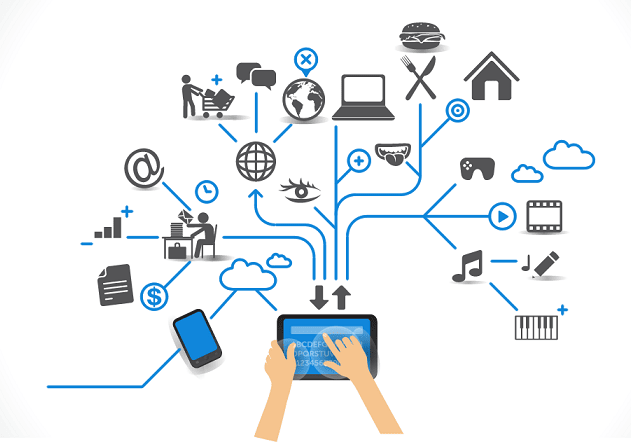
\includegraphics[scale=0.75]{Plataforma_internet.png}
	\caption[{Διαδίκτυο}]{Διαδίκτυο \textbf{Πηγή:} \cite{fig_Plataforma_internet}}
	\label{fig:Plataforma_internet}
\end{figure}

Το Διαδίκτυο μπορεί να χρησιμοποιηθεί για σχεδόν κάθε σκοπό που εξαρτάται από την πληροφορία, και όποιος έχει την δυνατότητα να συνδεθεί σε ένα από τα δίκτυα που το συνθέτουν, έχει πρόσβαση σε αυτό. Υποστηρίζει την ανθρώπινη επικοινωνία μέσω των κοινωνικών μέσων, του ηλεκτρονικού ταχυδρομείου (e-mail), των "chat rooms", και επιτρέπει στους ανθρώπους να συνεργάζονται είτε σύγχρονα, είτε ασύγχρονα σε πολλά διαφορετικά μέρη του κόσμου. Υποστηρίζει την πρόσβαση σε ψηφιακές πληροφορίες μέσω πολλών εφαρμογών, συμπεριλαμβανομένου του Παγκόσμιου Ιστού. Το Διαδίκτυο έχει διαδραματίσει σημαντικό ρόλο στην ανάπτυξη ενός μεγάλου και αυξανόμενου αριθμού "ηλεκτρονικών επιχειρήσεων" (συμπεριλαμβανομένων και των θυγατρικών των παραδοσιακών εταιρειών) που χρησιμοποιούν το Διαδίκτυο για το μεγαλύτερο μέρος των πωλήσεων και των υπηρεσιών τους.

\subsection{Παγκόσμιος Ιστός}
Αν και μερικές φορές χρησιμοποιούνται εναλλακτικά, οι όροι Διαδίκτυο και Παγκόσμιος Ιστός δεν σημαίνουν το ίδιο. Ο Παγκόσμιος Ιστός είναι μία από τις κύριες υπηρεσίες που παρέχονται μέσω του Διαδικτύου, ενώ ο όρος "Διαδίκτυο" αναφέρεται σε ολόκληρο το παγκόσμιο σύστημα επικοινωνίας, που περιλαμβάνει το υλικό και την υποδομή. Πιο επίσημα, ο Παγκόσμιος Ιστός μπορεί να οριστεί ως ένα σύστημα τεχνικοκοινωνικής αλληλεπίδρασης. Ένα σύστημα που βελτιώνει την ανθρώπινη διάνοια, την επικοινωνία και τη συνεργασία αναφέρεται ως τεχνοκοινωνικό σύστημα. Οι πληροφορίες που δημιουργούνται στον Παγκόσμιο Ιστό από τους χρήστες του μπορούν να αποθηκεύονται στο Διαδίκτυο. Υπάρχουν διάφοροι ιστότοποι στον Παγκόσμιο Ιστό, καθένας από τους οποίους έχει τη δική του διεύθυνση URL (Uniform Resource Locator). Η διεύθυνση URL έχει τη μορφή http://www.example.com. Το http συνιστά τη βάση δεδομένων επικοινωνίας για τον Παγκόσμιο Ιστό, το www πρόκειται για το World Wide Web, το οποίο είναι ένα πληροφοριακό σύστημα όπου τα έγγραφα και άλλοι δικτυακοί τόποι αναγνωρίζονται από τις διευθύνσεις URL τους, το example δηλώνει το όνομα του δικτυακού τόπου (domain name) και το com υποδεικνύει την περιοχή στην οποία ανήκει ο δικτυακός τόπος ή τον τύπο του δικτυακού τόπου \cite{aghaei2012evolution}.

\subsection{Εφαρμογή Ιστού}
Μια Εφαρμογή Web (Ιστού) συνιστά μια εφαρμογή που διανέμεται μέσω του Διαδικτύου με τη χρήση ενός προγράμματος περιήγησης και διατηρείται σε έναν απομακρυσμένο διακομιστή. Εξ ορισμού, οι υπηρεσίες διαδικτύου είναι Εφαρμογές Ιστού και πολλοί ιστότοποι -αν και όχι όλοι- περιέχουν τέτοιες εφαρμογές. Οι Εφαρμογές Ιστού μπορούν να δημιουργηθούν για ένα ευρύ φάσμα σκοπών και να χρησιμοποιηθούν από ανθρώπους ή οργανισμούς για πολλά διαφορετικά πράγματα. Το webmail, οι ηλεκτρονικές αριθμομηχανές και οι ιστότοποι ηλεκτρονικών αγορών είναι μερικά παραδείγματα συχνά χρησιμοποιούμενων Εφαρμογών Ιστού. Αν και η πλειονότητα των εφαρμογών ιστού είναι προσβάσιμες από οποιοδήποτε πρόγραμμα περιήγησης, ορισμένες είναι προσβάσιμες μόνο από ένα συγκεκριμένο πρόγραμμα περιήγησης \cite{Web_Apps}.

\section{Τεχνικές Προγραμματισμού}

\subsection{Αντικειμενοστρεφής Προγραμματισμός}
Ο αντικειμενοστρεφής προγραμματισμός (Object Oriented Programming / OOP), αποτελεί πρότυπο στην ανάπτυξη εφαρμογών, σε οποιαδήποτε γλώσσα. Βασίζεται στις ιδέες των κλάσεων και των αντικειμένων. Χρησιμοποιείται για την οργάνωση του λογισμικού σε απλές, επαναχρησιμοποιήσιμες κλάσεις σχεδίων κώδικα, οι οποίες στη συνέχεια χρησιμοποιούνται για τη δημιουργία ξεχωριστών περιπτώσεων αντικειμένων. Οι γλώσσες αντικειμενοστρεφούς προγραμματισμού JavaScript, C++, Java, Python και PHP είναι μερικά μόνο παραδείγματα \cite{smith2011object}.

Μια κλάση είναι ένα γενικευμένο πρότυπο που μπορεί να χρησιμοποιηθεί για τη δημιουργία πιο εξειδικευμένων, συγκεκριμένων πραγμάτων. Ευρείες κατηγορίες με κοινές ιδιότητες αναπαρίστανται συχνά με τη χρήση κλάσεων. Αυτές οι κλάσεις καθορίζουν τα χαρακτηριστικά μιας περίπτωσης τύπου, όπως το χρώμα, αλλά όχι την τιμή αυτών των χαρακτηριστικών για ένα συγκεκριμένο αντικείμενο.

Οι κλάσεις μπορούν επίσης να περιλαμβάνουν μεθόδους, οι οποίες είναι ειδικές λειτουργίες προσβάσιμες μόνο από αντικείμενα αυτού του είδους. Αυτές οι συναρτήσεις, οι οποίες ορίζονται εντός της κλάσης, εκτελούν ορισμένες χρήσιμες ενέργειες για το συγκεκριμένο είδος αντικειμένου.

Η δημιουργία μοναδικών αντικειμένων ακολουθεί το σχέδιο που παρέχουν τα πρότυπα κλάσεων. Κάθε αντικείμενο μπορεί να έχει διαφορετική τιμή για κάθε μία από τις δηλωμένες ιδιότητες της κλάσης \cite{Doherty_2020}.


\subsection{Αρχιτεκτονική MVC}
Το MVC είναι ένα αρχιτεκτονικό πρότυπο, το οποίο υποδηλώνει ότι ελέγχει ολόκληρο το σχεδιασμό της εφαρμογής. Παρόλο που αναφέρεται συχνά ως πρότυπο σχεδίασης, αυτό μπορεί να είναι ανακριβές, διότι τα πρότυπα σχεδίασης χρησιμοποιούνται για την αντιμετώπιση ορισμένων τεχνικών ζητημάτων, αλλά τα πρότυπα αρχιτεκτονικής αντιμετωπίζουν αρχιτεκτονικά ζητήματα, έχοντας αντίκτυπο σε ολόκληρο τον σχεδιασμό του προγράμματός μας \cite{Svirca_2020}.

Όπως φαίνεται και στο σχήμα \ref{fig:mvc-arch}, υπάρχουν τρία βασικά μέρη σε αυτό: το Μοντέλο, η Προβολή και ο Ελεγκτής. Καθένα από αυτά είναι υπεύθυνο για συγκεκριμένες εργασίες.

\begin{figure}[h]
	\centering
	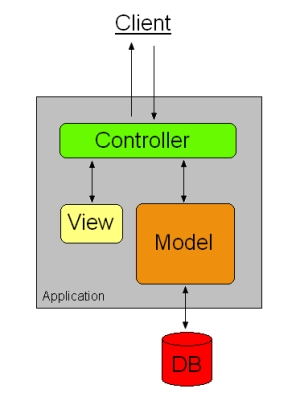
\includegraphics[scale=0.75]{MVC_Diagram_3.jpg}
	\caption[{Διάγραμμα Αρχιτεκτονικής MVC}]{Διάγραμμα Αρχιτεκτονικής MVC \textbf{Πηγή:} \cite{fig_MVC_Diagram_3}}
	\label{fig:mvc-arch}
\end{figure}

Δεδομένου ότι ένα μοντέλο θεωρείται ότι βρίσκεται στο χαμηλότερο επίπεδο, είναι υπεύθυνο για τη διατήρηση των δεδομένων. Ο χειρισμός δεδομένων με βάση τη λογική είναι ουσιαστικά ο τρόπος με τον οποίο χειρίζεται τα δεδομένα. Εφόσον το μοντέλο και η βάση δεδομένων είναι πραγματικά συνδεδεμένα, ό,τι κάνετε με τα δεδομένα θα λειτουργεί. Στο συστατικό μοντέλο, τα δεδομένα προστίθενται ή ανακτώνται. Επειδή ο ελεγκτής δεν επικοινωνεί ποτέ από μόνος του με τη βάση δεδομένων, αντιδρά σε ερωτήματα από τον ελεγκτή. Το μοντέλο επικοινωνεί συνεχώς με τη βάση δεδομένων πριν παράσχει στον ελεγκτή τις απαιτούμενες πληροφορίες. Αξίζει να σημειωθεί ότι το μοντέλο και η προβολή δεν είχαν ποτέ άμεση επικοινωνία.

Το στοιχείο προβολής χειρίζεται την αναπαράσταση δεδομένων. Στην πραγματικότητα, δημιουργεί τη διεπαφή χρήστη (UI) για τον χρήστη. Επομένως, όταν σκέφτεστε το στοιχείο προβολής σε εφαρμογές ιστού, σκεφτείτε απλώς το τμήμα HTML/CSS. Τα δεδομένα που συγκεντρώνει το συστατικό μοντέλο για τις προβολές λαμβάνονται μέσω του ελεγκτή και όχι απευθείας, επομένως η προβολή επικοινωνεί μόνο με τον ελεγκτή.

Ως το συστατικό που παρέχει τη σύνδεση μεταξύ των προβολών και του μοντέλου, ο ελεγκτής αναφέρεται ως ο "κύριος ρόλος", δεδομένου ότι λειτουργεί ως ενδιάμεσος. Ο ελεγκτής χρειάζεται μόνο να δίνει οδηγίες στο μοντέλο - δεν χρειάζεται να ανησυχεί για το χειρισμό της λογικής των δεδομένων. Αφού επεξεργαστεί τα δεδομένα που έχει λάβει από το μοντέλο, τα στέλνει στην όψη και δίνει οδηγίες στον χρήστη για τον τρόπο απεικόνισής τους. Οι προβολές και τα μοντέλα δεν μπορούν να συνομιλούν άμεσα \cite{tutorials_2022}.

\subsection{RESTful API}
Η μεταφορά κατάστασης παρουσίασης (REpresentational State Transfer), κοινώς γνωστή ως REST, είναι ένας αρχιτεκτονικός σχεδιασμός για κατανεμημένα συστήματα υπερμέσων. Παρουσιάστηκε για πρώτη φορά στη διάσημη διατριβή του Roy Fielding από το 2000.
Οι κατευθυντήριες έννοιες και οι περιορισμοί του REST είναι παρόμοιοι με εκείνους άλλων αρχιτεκτονικών στυλ. Εάν μια διεπαφή υπηρεσίας θέλει να αναφέρεται ως RESTful, πρέπει να τηρεί αυτά τα πρότυπα \cite{Gupta_2020}.

\begin{figure}[h]
	\centering
	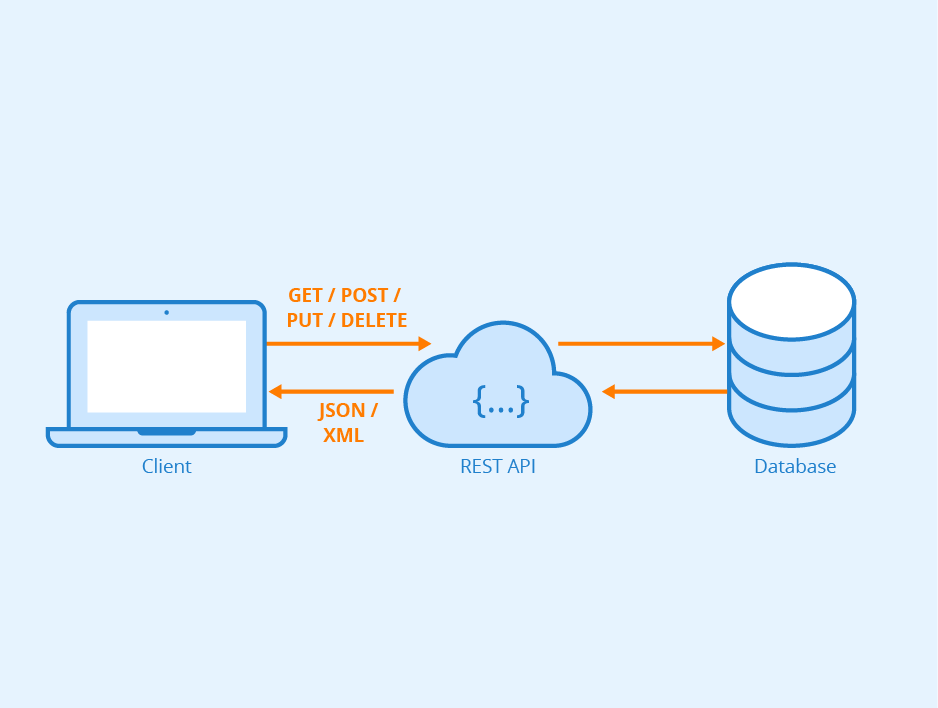
\includegraphics[scale=0.75]{Rest-API.png}
	\caption[{REST API}]{REST API \textbf{Πηγή:} \parencite{fig_Rest_API}}
	\label{fig:rest_api}
\end{figure}

Ένα σύνολο ορισμών και πρωτοκόλλων, γνωστό ως API, χρησιμοποιείται για τη δημιουργία και την ενσωμάτωση λογισμικού εφαρμογών. Μερικές φορές αναφέρεται ως σύμβαση μεταξύ ενός παρόχου πληροφοριών και ενός χρήστη αυτών των πληροφοριών, η οποία περιγράφει το περιεχόμενο που ο καταναλωτής (η κλήση) και ο παραγωγός υποχρεούνται να παραδώσουν (η απάντηση). Το API περιγράφει τον τρόπο με τον οποίο ένας προγραμματιστής θα πρέπει να σχεδιάσει ένα πρόγραμμα που ζητά υπηρεσίες από ένα λειτουργικό σύστημα ή μια άλλη εφαρμογή. 

Ένα API μπορεί να θεωρηθεί ως μεσάζων μεταξύ των χρηστών ή των πελατών και των πόρων ή των επιγραμμικών υπηρεσιών στις οποίες προσπαθούν να έχουν πρόσβαση. Επιπλέον, παρέχει σε μια εταιρεία έναν μηχανισμό για την κοινή χρήση περιουσιακών στοιχείων και δεδομένων, διατηρώντας παράλληλα την αυθεντικοποίηση, τον έλεγχο και την ασφάλεια - αποφασίζοντας ποιος έχει πρόσβαση σε τι \cite{RedHat_2020}. 

Ένα RESTful API βασίζεται στην αναπαραστατική μεταφορά κατάστασης (REST), ένα αρχιτεκτονικό στυλ και μια προσέγγιση επικοινωνίας που χρησιμοποιείται συχνά στην κατασκευή υπηρεσιών ιστού. Είναι επίσης γνωστό ως RESTful υπηρεσία ιστού ή REST API.

Γενικά, η τεχνολογία REST προτιμάται έναντι άλλων, συγκρίσιμων τεχνολογιών. Αυτό συμβαίνει συχνά, καθώς η REST απαιτεί μικρότερο εύρος ζώνης και, ως εκ τούτου, είναι πιο κατάλληλη για την αποτελεσματική χρήση του διαδικτύου. Επιπλέον, γλώσσες υπολογιστών όπως η JavaScript ή η Python μπορούν να χρησιμοποιηθούν για τη δημιουργία RESTful API \cite{Gillis_2020}.

\section{Γλώσσες Προγραμματισμού Ιστού}

\subsection{HTML}
Η HTML (Hyper Text Markup Language - Γλώσσα Σήμανσης Υπερκειμένου) αποτελεί την βασική γλώσσα για την κατασκευή ενός ιστοχώρου. Δεν θεωρείται γλώσσα προγραμματισμού, αλλά αποτελεί μία περιγραφική γλώσσα (markup language) η οποία περιέχει οδηγίες προς τους web browsers. Οι web browsers αφού διαβάσουν τις οδηγίες αυτές, τις μεταφράζουν στις κατάλληλες εντολές για να δημιουργηθεί το οπτικό περιεχόμενο που θα παρουσιαστεί στον χρήστη. Η παραπάνω διαδικασία επιτυγχάνεται με την βοήθεια των HTML elements, τα οποία οριοθετούνται από ετικέτες (tags). Οι ετικέτες είναι γράμματα ή λέξεις, τα οποία περικλείουν γωνιώδεις αγκύλες και υπάρχουν ανά ζεύγη. Χωρίζονται σε tags έναρξης, τα οποία σηματοδοτούν την έναρξη μιας εντολής, και σε tags λήξης, τα οποία σηματοδοτούν την λήξη της εντολής, με μερικές εξαιρέσεις. Οι ετικέτες λήξης διαχωρίζονται από τις ετικέτες έναρξης με μία πλάγια γραμμή '/'. Ένα βασικό παράδειγμα ετικέτας είναι το: <html>...</html>, ανάμεσα στις ετικέτες περικλείεται κείμενο ή ακόμη και άλλες εσωτερικές ετικέτες (εμφωλευμένα tags). Ορισμένες βασικές ετικέτες παρατίθενται στον πίνακα \ref{tbl:html_basic_elements}.

\begin{longtable}{|p{0.2\linewidth}|p{0.7\linewidth}|} 
	\caption{Βασικά στοιχεία HTML} \label{tbl:html_basic_elements} \\
	\hline
	\endfirsthead
	\caption[{}]{Βασικά στοιχεία HTML (συνέχεια)} \\ 
	\endhead \endfoot 
	\textless{}html\textgreater{}...\textless{}/html\textgreater{} & Η αρχή και το τέλος του HTML αρχείου \\ \hline
	\textless{}!DOCTYPE\textgreater{} & Η οδηγία που καθορίζει την έκδοση της HTML που χρησιμοποιείται \\ \hline
	\textless{}head\textgreater{}...\textless{}/head\textgreater{} & Οι σχετικές πληροφορίες με το έγγραφο (όπως η γλώσσα, η κωδικοποίηση και τα μεταδεδομένα) \\ \hline
	\textless{}title\textgreater{}...\textless{}/title\textgreater{} & Ο τίτλος του αρχείου \\ \hline
	\textless{}body\textgreater{}...\textless{}/body\textgreater{} & Τα οπτικά στοιχεία του αρχείου \\ \hline
	\textless{}div\textgreater{}...\textless{}/div\textgreater{} & Ομαδοποίηση στοιχείων εντός ετικέτας \\ \hline
	\textless{}input\textgreater{}...\textless{}/input\textgreater{} & Ορισμός πεδίου εισαγωγής \\ \hline
	\textless{}!--...--\textgreater{} & Ορισμός σχολίων \\ \hline
	\textless{}form\textgreater{}...\textless{}/form\textgreater{} & Ορισμός φόρμας \\ \hline
	\textless{}button\textgreater{}...\textless{}/button\textgreater{} & Ορισμός κουμπιού \\ \hline
	\textless{}a\textgreater{}...\textless{}/a\textgreater{} & Ορισμός υπερσυνδέσμου \\ \hline
\end{longtable}

\subsection{CSS}
Η CSS αποτελεί μία γλώσσα επικαλυπτόμενων στυλ μορφοποίησης (Cascading Style Sheets) και όπως η HTML δεν θεωρείται καθαρή γλώσσα προγραμματισμού. Συντελεί στον διαχωρισμό των εντολών εμφάνισης από τις εντολές του περιεχομένου της ιστοσελίδας. Χρησιμοποιείται για τη μορφοποίηση οποιασδήποτε ετικέτας HTLM και τη δημιουργία ενός αποτελέσματος πιο όμορφου οπτικά για τον χρήστη. Η σύνταξη μιας εντολής στην CSS αποτελείται από τρία κύρια στοιχεία: το στοιχείο που θα τροποποιηθεί, τις ιδιότητες του στοιχείου που θα επηρεαστούν και η νέα τιμή των ιδιοτήτων. Στον πίνακα \ref{tbl:css_basic_elements} αναφέρεται ένα παράδειγμα του τρόπου σύνταξης μιας εντολής στην γλώσσα CSS.

\begin{table}[h]
	\caption{Στοιχεία εντολής CSS}
	\label{tbl:css_basic_elements}
	\centering
	\begin{tabular}{|l|}
		\hline
		\begin{tabular}[c]{@{}l@{}}
			p \{ \\ \quad 
			font-family: Calibri; \\ \quad 
			color: \#1B1811; \\ \quad 
			text-align: left; \\ \}
		\end{tabular} \\ \hline
	\end{tabular}
\end{table}

Όπως φαίνεται στον πίνακα \ref{tbl:css_basic_elements}, το στοιχείο p αποτελεί την ετικέτα της παραγράφου στην HTML και ονομάζεται επιλογέας (css selector). Τα font-family, color και text-align είναι οι ιδιότητες της εντολής CSS και δείχνουν τα στοιχεία του επιλογέα τα οποία θα τροποποιηθούν. Ο διαχωρισμός των ιδιοτήτων από τις νέες τιμές που θα λάβουν σηματοδοτείται με την άνω και κάτω τελεία (:), στης οποίας το αριστερό μέρος βρίσκονται οι ιδιότητες και στο δεξί οι νέες τιμές τους.

\subsection{JavaScript \& Ajax}
Η JavaScript είναι μια γλώσσα προγραμματισμού σεναρίου (scripting language), η οποία εκτελείται από τους περιηγητές ιστών (web browsers) χρησιμοποιώντας έναν σχετικό διερμηνευτή (Interpreter). Στόχο της αποτελεί η βελτίωση της εμπειρίας χρήσης. Με την JavaScript υπάρχει η δυνατότητα προσθήκης ή αφαίρεσης HTML στοιχείων και CSS κανόνων καθώς και η τροποποίηση ιδιοτήτων HTLM στοιχείων με την μεταβολή στις τιμές τους. Αν και η JavaScript αποτελεί μια γλώσσα προγραμματισμού με το Client-Side χαρακτηριστικό, τον τελευταίο καιρό γίνεται χρήση της και από την πλευρά των υπολογιστών εξυπηρετητών.

Η Ajax (Asynchronous JavaScript and XML) αποτελείται από τον συνδυασμό των τεχνολογιών JavaScript και XML. Είναι μία τεχνολογία, η οποία προσδίδει διαδραστικές δυνατότητες σε μία ιστοσελίδα. Μέσω της Ajax γίνεται εφικτή η ανανέωση μέρους της ιστοσελίδας (στο παρασκήνιο θα γίνει επικοινωνία της τεχνολογίας με τον server, ο οποίος θα λάβει τα δεδομένα που ζητήθηκαν και με τη σειρά του θα τα εμφανίσει στον χρήστη), χωρίς να χρειαστεί να γίνει ανανέωση (refresh) ολόκληρης της ιστοσελίδας.

\subsection{PHP}
Η PHP ορίζεται ως μία αντικειμενοστρεφής γλώσσα προγραμματισμού γενικής χρήσης (παλαιότερα αποτελούσε γλώσσα προγραμματισμού σεναρίου), η οποία χρησιμοποιείται κυρίως για την ανάπτυξη διαδικτυακών εφαρμογών (web apps), δηλαδή αποτελεί την κατάλληλη γλώσσα για την δημιουργία ιστοχώρων με δυναμικό περιεχόμενο. Διατίθεται σε δύο μορφές, σε μορφή πηγαίου κώδικα και σε δυαδική μορφή και οι δύο αυτές μορφές έχουν ελεύθερη πρόσβαση. Η PHP χρησιμοποιείται για τον χειρισμό λειτουργιών και εργασιών τις οποίες θα υλοποιήσει και όχι για την οπτική διαμόρφωση μίας ιστοσελίδας.

Επομένως, ο χρήστης λαμβάνει τα αποτελέσματα του σεναρίου (στον browser ως απλές σελίδες HTLM) και όχι τον κώδικα, ο οποίος εκτελείται στον server με τη χρήση του αντίστοιχου διερμηνευτή (interpreter) της κάθε γλώσσας. Ο διερμηνευτής, αφού διαβάσει τον κώδικα, εκτελεί τις δηλώσεις της γλώσσας ανά βήμα και τις μετατρέπει σε εκτελέσιμο κώδικα για το υπολογιστικό σύστημα.

Αναλυτικότερα, η PHP έχει την ικανότητα να δημιουργήσει, γράψει, διαβάσει, ανοίξει, κλείσει και διαγράψει αρχεία στη Βάση Δεδομένων. Υποστηρίζει ένα ευρύ φάσμα Βάσεων Δεδομένων, καθώς επίσης είναι δωρεάν και αρκετά εύκολη στην εκμάθηση, ενώ ταυτόχρονα είναι συμβατή και μπορεί να τρέξει σε οποιαδήποτε πλατφόρμα, όπως για παράδειγμα Windows, Mac OS X, Linux, Unix κ.α. Ένα αρχείο PHP (έγγραφο κειμένου αποθηκευμένο με την κατάληξη .php) είναι δυνατό να περιέχει εκτός από τον κώδικα PHP και κώδικα HTLM, CSS και JavaScript.

Ορισμένες βασικές συναρτήσεις της PHP παρατίθενται στον πίνακα \ref{tbl:php_basic_functions}.

\begin{longtable}{|p{0.2\linewidth}|p{0.7\linewidth}|} 
	\caption{Βασικές συναρτήσεις της PHP} \label{tbl:php_basic_functions} \\
	\hline
	\endfirsthead
	\caption[{}]{Βασικές συναρτήσεις της PHP (συνέχεια)} \\ 
	\endhead \endfoot 
	htmlspecialchars() & Μετατροπή ειδικών χαρακτήρων σε οντότητες HTML \\ \hline
	explode() & Μετατροπή μιας συμβολοσειράς σε πίνακα με χρήση ενός διαχωριστικού χαρακτήρα \\ \hline
	rand() & Επιστροφή ενός τυχαίου αριθμού \\ \hline
	str\_replace() & Εύρεση και αντικατάσταση ενός μοτίβου σε μια συμβολοσειρά \\ \hline
	date() & Επιστροφή μιας μορφοποιημένης ημερομηνίας \\ \hline
	strlen() & Επιστροφή του μήκους μιας συμβολοσειράς \\ \hline
	count() & Επιστροφή του αριθμού των στοιχείων ενός πίνακα \\ \hline
	array\_unique() & Απαλοιφή διπλότυπων στοιχείων ενός πίνακα \\ \hline
	print\_r() & Εκτύπωση μεταβλητής \\ \hline
	echo & Εκτύπωση μίας ή περισσότερων συμβολοσειρών \\ \hline
\end{longtable}

\subsection{SQL}
Η Structured Query Language (SQL) \cite{Loshin_2022}, μία τυποποιημένη γλώσσα προγραμματισμού, χρησιμοποιείται για τη διαχείριση σχεσιακών βάσεων δεδομένων και την εκτέλεση διαφόρων πράξεων στα δεδομένα που περιέχουν. Από την ίδρυσή της τη δεκαετία του 1970, η SQL χρησιμοποιείται ευρέως από διαχειριστές βάσεων δεδομένων καθώς και από προγραμματιστές που δημιουργούν σενάρια για την ολοκλήρωση δεδομένων και από αναλυτές δεδομένων που κατασκευάζουν και εκτελούν αναλυτικά ερωτήματα.

Με τη βοήθεια της ευέλικτης γλώσσας SQL, οι χρήστες μπορούν να λαμβάνουν, να αποθηκεύουν, να επεξεργάζονται και να διαγράφουν δεδομένα, καθώς και να δημιουργούν, να τροποποιούν και να αφαιρούν αντικείμενα βάσεων δεδομένων (όπως πίνακες, στήλες, διαδικασίες και χρήστες), καθώς και να δίνουν και να ανακαλούν προνόμια χρηστών και να ομαδοποιούν δηλώσεις σε συναλλαγές. Μια δήλωση που ζητά δεδομένα από τη βάση δεδομένων αναφέρεται ως ερώτημα και μια εντολή SQL είναι γνωστή ως δήλωση. Στις εντολές SQL περιλαμβάνονται προγνωστικά (όπως LIKE, BETWEEN, EXISTS), τελεστές (όπως AND, OR, NOT), ποσοδείκτες (όπως ANY, ALL, UNION), συναρτήσεις (όπως COUNT, SUM, AVG) και προτάσεις (όπως SELECT, FROM, WHERE). Όταν δεν είναι σημαντικό να γίνει διάκριση μεταξύ, για παράδειγμα, των ρητρών και των κατηγορημάτων, αναφερόμαστε σε αυτά ως έννοιες συλλογικά.
Η γλώσσα χειρισμού δεδομένων (DML, π.χ. SELECT, INSERT, UPDATE, DELETE) και η γλώσσα ορισμού δεδομένων (DDL, π.χ. CREATE, ALTER, DROP) είναι οι δύο υπογλώσσες της SQL που χρησιμοποιούνται συχνότερα \cite{taipalus2020sql}.
 
Τα δεδομένα αποθηκεύονται, ανακτώνται και αναλύονται με τη χρήση λογισμικού που ονομάζεται σύστημα διαχείρισης βάσεων δεδομένων (DBMS). Οι χρήστες μπορούν να δημιουργούν, να διαβάζουν, να ενημερώνουν και να διαγράφουν δεδομένα σε βάσεις δεδομένων χρησιμοποιώντας ένα DBMS, το οποίο λειτουργεί ως διεπαφή μεταξύ αυτών και των βάσεων δεδομένων. Η ασφάλεια των δεδομένων, η ακεραιότητα των δεδομένων, η ταυτόχρονη χρήση και οι τυποποιημένες πρακτικές διαχείρισης δεδομένων βοηθούνται από αυτό.

Τα μοντέλα δεδομένων, οι κατανομές βάσεων δεδομένων, ο αριθμός των χρηστών και άλλοι παράγοντες μπορούν να χρησιμοποιηθούν για την κατηγοριοποίηση των συστημάτων διαχείρισης βάσεων δεδομένων. Οι σχεσιακές, κατανεμημένες, ιεραρχικές, αντικειμενοστραφείς και δικτυακές μορφές λογισμικού DBMS είναι οι πιο δημοφιλείς \cite{DBMS}.

Στα συστήματα διαχείρισης σχεσιακών βάσεων δεδομένων (RDBMS), η SQL χρησιμοποιείται για τις ακόλουθες εργασίες: αλλαγή των δομών των πινάκων και των δεικτών της βάσης δεδομένων, προσθήκη, ενημέρωση και διαγραφή γραμμών δεδομένων και ανάκτηση υποσυνόλων πληροφοριών. Οι πληροφορίες αυτές μπορούν να χρησιμοποιηθούν για την επεξεργασία συναλλαγών, εφαρμογές ανάλυσης και άλλες εφαρμογές που απαιτούν αλληλεπίδραση με μια σχεσιακή βάση δεδομένων.

\section{Πλαίσια και Βιβλιοθήκες Προγραμματισμού Ιστού}

\subsection{Bootstrap}
Μια βιβλιοθήκη HTML, CSS και JS με έμφαση στη βελτιστοποίηση της διαδικασίας ανάπτυξης ιστοσελίδων ονομάζεται Bootstrap (σε αντίθεση με τις εφαρμογές ιστού). Το Bootstrap είναι ένα δωρεάν και ανοικτού κώδικα πλαίσιο CSS που δημιουργήθηκε αρχικά από το Twitter και σήμερα αναπτύσσεται από την ομάδα Bootstrap στο GitHub για την ανάπτυξη front-end ιστοσελίδων που δίνει προτεραιότητα στις κινητές συσκευές. Προσφέρει πρότυπα σχεδίασης HTML, CSS και (προαιρετικά) JavaScript για τυπογραφία, φόρμες, κουμπιά, πλοήγηση και άλλα στοιχεία διεπαφής \cite{Bootstrap}. 

Ο κύριος στόχος της προσθήκης του σε ένα έργο ιστού είναι η εφαρμογή των επιλογών χρώματος, μεγέθους, γραμματοσειράς και διάταξης του Bootstrap σε αυτό το έργο. Ως εκ τούτου, ο κύριος καθοριστικός παράγοντας είναι το κατά πόσον αυτές οι επιλογές αρέσουν στους υπεύθυνους προγραμματιστές. Όλα τα στοιχεία HTML έχουν βασικές δηλώσεις στυλ μόλις το Bootstrap εισαχθεί σε ένα έργο. 

Ως αποτέλεσμα, τα κείμενα, οι πίνακες και τα στοιχεία φόρμας εμφανίζονται με συνέπεια σε όλα τα προγράμματα περιήγησης ιστού. Προκειμένου να εξατομικεύσουν περαιτέρω την εμφάνιση του περιεχομένου τους, οι προγραμματιστές μπορούν να κάνουν χρήση των κλάσεων CSS που ορίζονται στο Bootstrap. Για παράδειγμα, το Bootstrap προσφέρει ενσωματωμένη υποστήριξη για ανοιχτόχρωμους και σκούρους πίνακες, επικεφαλίδες σελίδων, μεγαλύτερα pull quotes και κείμενο με υπογράμμιση \cite{bootstrap_2}.

Επιπλέον, το Bootstrap περιλαμβάνει μια σειρά από στοιχεία JavaScript που μπορούν να χρησιμοποιηθούν ανεξάρτητα από άλλα πλαίσια, όπως το jQuery. Προσφέρουν επιπλέον στοιχεία UI, όπως πλαίσια διαλόγου, tooltips, μπάρες προόδου, drop-down μενού και καρουσέλ \cite{gaikwad2019review}. Κάθε στοιχείο Bootstrap αποτελείται από ένα πλαίσιο HTML, δηλώσεις CSS και περιστασιακά από συμπληρωματικό κώδικα JavaScript. Ταυτόχρονα, αυξάνουν τη λειτουργικότητα μερικών ήδη υπαρχόντων στοιχείων διεπαφής, όπως η λειτουργία αυτόματης συμπλήρωσης για τα πεδία εισαγωγής.

\subsection{CodeIgniter}
Ένα πλαίσιο ανάπτυξης εφαρμογών MVC, ή εργαλειοθήκη, που ονομάζεται CodeIgniter, είναι διαθέσιμο για προγραμματιστές ιστοσελίδων PHP. Προσφέροντας μια ολοκληρωμένη συλλογή βιβλιοθηκών για συχνά εκτελούμενες λειτουργίες, καθώς και μια φιλική προς το χρήστη διεπαφή και μια λογική δομή πρόσβασης, στοχεύει να κάνει τη δημιουργία έργων σημαντικά ταχύτερη από τη συγγραφή κώδικα από το μηδέν. Το CodeIgniter προσπαθεί να γράφει όσο το δυνατόν λιγότερο κώδικα για την ολοκλήρωση μιας εργασίας \cite{Jackson_2020}.

Πρόκειται για ένα πλαίσιο με αμελητέες απαιτήσεις διαμόρφωσης. Προσφέρει εξαιρετικές επιδόσεις, διαθέτει λεπτομερή, σαφή τεκμηρίωση και δεν απαιτεί τη χρήση της γραμμής εντολών ή την τήρηση αυστηρών οδηγιών κωδικοποίησης. Αποφεύγει την πολυπλοκότητα και ευνοεί τις απλές διορθώσεις \cite{CodeIgniter_intro}.

\subsection{Swagger - OpenAPI}
Το Swagger είναι μια συλλογή οδηγιών, απαιτήσεων και πόρων ανοικτού κώδικα για τη δημιουργία και τον ορισμό RESTful APIs, τα οποία υλοποιούν τις προδιαγραφές του OpenAPI. Το έργο ξεκίνησε το 2011 από τον Tony Tam, ο οποίος εργαζόταν στη δημιουργία εργαλείων για τον ιστότοπο λεξικού Wordnik και πλέον συντηρείται από την SmartBear Software. Οι προγραμματιστές μπορούν να γράφουν διαδραστική, αναγνώσιμη από μηχανήματα και ανθρώπους τεκμηρίωση API χρησιμοποιώντας το πλαίσιο Swagger \cite{Swagger_2022}.

Πληροφορίες όπως υποστηριζόμενες λειτουργίες, παράμετροι και έξοδοι, ανάγκες εξουσιοδότησης, προσβάσιμα τελικά σημεία και απαιτούμενη αδειοδότηση περιλαμβάνονται συχνά στις προδιαγραφές API. Ζητώντας από το API να παραδώσει ένα αρχείο τεκμηρίωσης από τις επισημάνσεις του, το Swagger μπορεί να παράγει αυτόματα αυτές τις πληροφορίες από τον πηγαίο κώδικα.

Οι χρήστες μπορούν να δημιουργούν, να τεκμηριώνουν, να δοκιμάζουν και να καταναλώνουν RESTful υπηρεσίες ιστού με τη βοήθεια του Swagger. Εφαρμόζεται τόσο σε μεθοδολογίες ανάπτυξης API από πάνω προς τα κάτω όσο και από κάτω προς τα πάνω. Το Swagger μπορεί να χρησιμοποιηθεί για τη δημιουργία ενός API στην προσέγγιση top-down ή "design-first", πριν αναπτυχθεί οποιοσδήποτε κώδικας. Η τεκμηρίωση παράγεται από το Swagger χρησιμοποιώντας τον κώδικα που δημιουργείται για ένα API στην προσέγγιση "από κάτω προς τα πάνω" ή "code-first" \cite{Swagger_2019}.

\section{Τεχνολογίες Ανάπτυξης Λογισμικού}

\subsection{Jetbrains PhpStorm}
Κατασκευασμένο από την τσεχική εταιρεία JetBrains, το PhpStorm είναι ένα ιδιόκτητο, διαπλατφορμικό IDE (ολοκληρωμένο περιβάλλον ανάπτυξης) για την PHP \cite{grigorev2014string}. Με on-the-fly ανάλυση κώδικα, πρόληψη σφαλμάτων και αυτοματοποιημένες αναδιαμορφώσεις για κώδικα PHP και JavaScript, το PhpStorm προσφέρει έναν επεξεργαστή για PHP, HTML και JavaScript. Η PHP υποστηρίζεται από τη συμπλήρωση κώδικα του PhpStorm, η οποία υποστηρίζει επίσης namespaces, closures, traits, generators, coroutines, τη λέξη-κλειδί finally, λίστες σε foreach και σύνταξη σύντομων πινάκων. Περιλαμβάνεται ένας πλήρης επεξεργαστής SQL με επεξεργάσιμα αποτελέσματα ερωτημάτων.

Για τη συγγραφή του PhpStorm χρησιμοποιείται η Java. Εγκαθιστώντας plugins που έχουν κατασκευαστεί για το PhpStorm ή δημιουργώντας τα δικά τους, οι χρήστες μπορούν να επεκτείνουν τη λειτουργικότητα του IDE. Επιπλέον, το λογισμικό αλληλεπιδρά με εξωτερικούς πόρους όπως το XDebug. Το PhpStorm περιέχει όλες τις δυνατότητες που υπάρχουν στο WebStorm. Τα πρόσθετα JavaScript είναι ήδη προεγκατεστημένα στο WebStorm \cite{PhpStorm_JetBrains}.

\subsection{Git}
Το Global Information Tracker (Git) είναι ένα σύστημα ελέγχου εκδόσεων (VCS) διαθέσιμο σε όλες τις κύριες πλατφόρμες ανάπτυξης μέσω μιας άδειας χρήσης ελεύθερου λογισμικού \cite{spinellis2012git}. Ορισμένα χαρακτηριστικά που μπορεί να βρεθούν στο git είναι η διευκόλυνση της κατανεμημένης ανάπτυξης μέσω πολλαπλών προγραμματιστών σε πολλαπλές τοποθεσίες, γεγονός που οδηγεί στην κλίμακα για τον χειρισμό των χιλιάδων προγραμματιστών που εργάζονται στα ίδια ή διαφορετικά μέρη ενός έργου. Η γρήγορη και αποδοτική απόδοση με τη χρήση τεχνικών "delta" και συμπίεσης, η διατήρηση της ακεραιότητας των δεδομένων με την κρυπτογραφική συνάρτηση κατακερματισμού (SHA1) και η επιβολή της λογοδοσίας. Επίσης, υποστηρίζει και ενθαρρύνει τη διακλαδισμένη και σε άλλες περιπτώσεις τη συγχωνευμένη ανάπτυξη. Μία ακόμη ιδιότητα του git είναι πως διαθέτει πλήρη αποθετήρια. Ένα αποθετήριο αποτελείται από πολλούς φακέλους και αρχεία τα οποία είναι προσβάσιμα από οποιονδήποτε έχει πρόσβαση στο ιδιωτικό αποθετήριο \cite{loeliger2012version}. 

Το Git διαθέτει έναν αριθμό από Graphical User Interfaces (GUI) πελάτες και ένας από αυτούς είναι το Gitkraken \cite{gitkrakenwhatisit}, το οποίο αποτελεί ένα γραφικό περιβάλλον διαχείρισης git αποθετηρίων. Χρησιμοποιείται για την εύκολη και αποτελεσματική διαχείριση, την δημιουργία, αλλά και την συγχώνευση των διακλαδώσεων. Διαθέτει την δυνατότητα να ενσωματώνεται με τον λογαριασμό GitHub ή Bitbucket ενός χρήστη, καθώς επίσης μπορεί να προσαρμοστεί εύκολα στον χώρο εργασίας του χρήστη.

Το GitHub είναι μία διαδικτυακή πλατφόρμα συνεργατικής φιλοξενίας κώδικα ανάπτυξης λογισμικού, που βασίζεται στο σύστημα ελέγχου εκδόσεων git. Μέσω του GitHub, οι προγραμματιστές έχουν την δυνατότητα να αντιγράψουν ένα αποθετήριο στον λογαριασμό τους (fork) και αφού πραγματοποιήσουν τις αλλαγές τους, τους δίνεται η δυνατότητα να προτείνουν  να ενσωματωθούν στο αρχικό αποθετήριο από τους συντηρητές του (pull request και merge). Οι προγραμματιστές μπορούν επίσης να ακολουθήσουν άλλους χρήστες, σχηματίζοντας έτσι ένα κύκλωμα ανταλλαγής πληροφοριών, όπου κάθε προγραμματιστής ενημερώνεται για εξελίξεις σχετικές με τα ενδιαφέροντα του \cite{kalliamvakou2014promises}. Εκτός από τις λειτουργίες του Git, το GitHub προσφέρει και μερικά επιπρόσθετα χαρακτηριστικά. Βοηθά στη διαχείριση της πρόσβασης και της συνεργασίας για έργα, παρέχοντας χαρακτηριστικά όπως είναι η παρακολούθηση σφαλμάτων, η διαχείριση των διαφόρων εργασιών και τα αιτήματα χαρακτηριστικών.

\section{Σύνοψη Κεφαλαίου 2}
Στο δεύτερο κεφάλαιο εξετάστηκαν οι μέθοδοι και οι γλώσσες προγραμματισμού που εφαρμόστηκαν για την επεξεργασία και την ανάπτυξη της διαδικτυακής εφαρμογής. Εκτός από τα εργαλεία προγραμματισμού, η διατριβή περιλαμβάνει επίσης μια λεπτομερή περιγραφή των εργαλείων λογισμικού που χρησιμοποιήθηκαν για την οργάνωση και την κατασκευή του πληροφοριακού συστήματος. 

Η κατασκευή της βάσης δεδομένων και η δομή και οργάνωση του συστήματος καλύπτονται στο επόμενο κεφάλαιο.


\chapter{Δομή \& Οργάνωση Συστήματος}
Σε αυτό το κεφάλαιο, περιγράφονται λεπτομερώς οι λειτουργικές και μη-λειτουργικές απαιτήσεις του συστήματος διαχείρισης εκκίνησης υπολογιστών μέσω δικτύου. Επίσης, αναλύονται τα δύο είδη χρηστών που έχουν πρόσβαση στο σύστημα και οι δυνατότητες που παρέχονται από τη διαδικτυακή εφαρμογή του συστήματος. Ακόμα, γίνεται ανάλυση του σχήματος της βάσης δεδομένων και επεξήγηση αρχείων του κώδικα, ο οποίος συντέλεσε στη δημιουργία του πληροφοριακού συστήματος.

\section{Ανάλυση Συστήματος}
Για την επίτευξη της ορθής ανάλυσης και σχεδίασης του συστήματος, είναι απαραίτητη η κατανόηση των λειτουργιών του και των δυνατοτήτων που προσφέρει στους χρήστες του. Οι χρήστες είναι είτε γενικοί διαχειριστές του συστήματος ή διαχειριστές συγκεκριμένων εργαστηρίων.

Οι γενικοί διαχειριστές του συστήματος, έχουν τη δυνατότητα να προσθέτουν, να αφαιρούν και να επεξεργάζονται στοιχεία υπολογιστών, οι οποίοι δύναται να εκκινηθούν δικτυακά, με μενού επιλογής λειτουργικού συστήματος παρεχόμενο από το σύστημα. Μπορούν ακόμα να προσθέτουν και να διαχειρίζονται εργαστήρια στα οποία βρίσκονται οι υπολογιστές. Μια ακόμη ενέργεια στην οποία μπορούν να προβούν οι γενικοί διαχειριστές, είναι να τοποθετούν τους υπολογιστές σε ομάδες, οι οποίες καθορίζουν τα μενού λειτουργικών συστημάτων που θα παρέχονται από το σύστημα, ανάλογα με την τρέχουσα ημερομηνία / ώρα. Τέλος, οι γενικοί διαχειριστές ορίζουν τα διαθέσιμα λειτουργικά συστήματα, φτιάχνουν μενού εκκίνησης με χρήση των ορισμένων λειτουργικών συστημάτων και ρυθμίζουν τις ημερομηνίες / ώρες στις οποίες το σύστημα θα παρέχει τα μενού λειτουργικών συστημάτων στις ομάδες υπολογιστών.

Οι διαχειριστές εργαστηρίων, μπορούν να πραγματοποιούν τι ίδιες ενέργειες με τους γενικούς διαχειριστές, αλλά μόνο για τα εργαστήρια που τους έχουν ανατεθεί. Μπορούν δηλαδή να διαχειρίζονται τους υπολογιστές, τις ομάδες υπολογιστών και τα μενού εκκίνησης των ομάδων, που βρίσκονται στα εργαστήρια για τα οποία έχουν λάβει δικαίωμα διαχείρισης από τους γενικούς διαχειριστές.
 
\section{Ανάλυση Απαιτήσεων}

\subsection{Λειτουργικές Προδιαγραφές}
Η διαδικτυακή εφαρμογή που υλοποιήθηκε, δίνει τη δυνατότητα στον χρήστη να διαχειρίζεται τα μενού λειτουργικών συστημάτων κατά τη δικτυακή εκκίνηση ομάδων υπολογιστών.

\subsection{Μη-Λειτουργικές Προδιαγραφές}
Η διαδικτυακή εφαρμογή έχει υλοποιηθεί ως ένα web interface που επικοινωνεί με τη βάση δεδομένων μέσω ενός CRUD (Create - Read - Update - Delete) API, με χρήση του CodeIgniter PHP Framework.

\section{Περιπτώσεις Χρήσης}
Στους πίνακες που ακολουθούν παρουσιάζονται οι περιπτώσεις χρήσης της πλατφόρμας.

\begin{table}[h]
	\caption{Σύνδεση στο σύστημα}
	\label{tab:use-case-login}
	\begin{tabular}{|p{0.2\linewidth}|p{0.7\linewidth}|}
		\hline
		Περιγραφή: & Ο τρόπος με τον οποίο συνδέεται ο χρήστης στην πλατφόρμα \\ \hline
		Χειριστές: & Γενικός Διαχειριστής Πλατφόρμας, Διαχειριστής Εργαστηρίου \\ \hline
		Προϋποθέσεις: & Ο χρήστης πρέπει να είναι εγγεγραμμένος στην πλατφόρμα \\ \hline
		Βασική ροή: & 
		\begin{enumerate}
			\item Ο χρήστης δεν έχει session cookie στον περιηγητή ιστού του
			\item Ο χρήστης εισάγει το όνομα χρήστη και το κωδικό του λογαριασμού του
			\item Επιβεβαιώνεται η επιτυχής εισαγωγή των στοιχείων και ο χρήστης συνδέεται στο σύστημα
		\end{enumerate} \\ \hline
		Εναλλακτικό σενάριο: & O χρήστης εισάγει εσφαλμένα στοιχεία, η πλατφόρμα απορρίπτει τη σύνδεση, εμφανίζει μήνυμα σφάλματος και ζητά από τον χρήστη να δοκιμάσει ξανά να εισαγάγει τα σωστά στοιχεία. \\ \hline
	\end{tabular}
\end{table}

\begin{table}[h]
	\caption{Εγγραφή χρήστη στο σύστημα}
	\label{tab:use-case-register}
	\begin{tabular}{|p{0.2\linewidth}|p{0.7\linewidth}|}
		\hline
		Περιγραφή: & Ο τρόπος με τον οποίο εγγράφονται οι χρήστες στην πλατφόρμα \\ \hline
		Χειριστές: & Ανώνυμος Χρήστης \\ \hline
		Προϋποθέσεις: & Καμία \\ \hline
		Βασική ροή: & 
		\begin{enumerate}
			\item Ο χρήστης συμπληρώνει τα στοιχεία του στη σελίδα εγγραφής
			\item Επιβεβαιώνεται η επιτυχής εισαγωγή των στοιχείων και γίνεται επαλήθευσή τους από client-side και server-side validators για την εξακρίβωση τύπου και πλήθους δεδομένων
			\item Επιβεβαιώνεται η επιτυχής εισαγωγή των στοιχείων και εισέρχεται στο σύστημα
		\end{enumerate} \\ \hline
		Εναλλακτικό σενάριο: & O χρήστης εισάγει εσφαλμένα στοιχεία, η πλατφόρμα απορρίπτει τη σύνδεση, εμφανίζει μήνυμα σφάλματος και ζητά από τον χρήστη να δοκιμάσει ξανά να εισαγάγει τα σωστά στοιχεία.                     \\ \hline
	\end{tabular}
\end{table}

\begin{table}[h]
	\caption{Επανέκδοση κωδικού}
	\label{tab:use-case-forgot-password}
	\begin{tabular}{|p{0.2\linewidth}|p{0.7\linewidth}|}
		\hline
		Περιγραφή: & Ο τρόπος με τον οποίο ο χρήστης δημιουργεί νέο κωδικό για τον λογαριασμό του σε περίπτωση που ξεχάσει τον παλιό \\ \hline
		Χειριστές: & Γενικός Διαχειριστής Πλατφόρμας, Διαχειριστής Εργαστηρίου \\ \hline
		Προϋποθέσεις: & Καμία \\ \hline
		Βασική ροή: & 
		\begin{enumerate}
			\item Ο χρήστης έχει ξεχάσει τον κωδικό του λογαριασμού του
			\item Ο χρήστης περιηγείται στο σημείο επανέκδοσης κωδικού πρόσβασης
			\item Εισάγει το όνομα χρήστη του στη φόρμα
			\item Λαμβάνει στο email του έναν ειδικό σύνδεσμο επανέκδοσης του κωδικού του
			\item Ακολουθεί τον σύνδεσμο και εισάγει τον νέο κωδικού του λογαριασμού του
			\item Συνδέεται στην πλατφόρμα με χρήση του νέου κωδικού του
		\end{enumerate} \\ \hline
		Εναλλακτικό σενάριο: & Αν ο χρήστης εισάγει λάθος όνομα χρήστη στο βήμα 3, δε θα λάβει το email επαναφοράς του κωδικού του. \\ \hline
	\end{tabular}
\end{table}

\begin{table}[h]
	\caption{Υπενθύμιση Ονόματος Χρήστη}
	\label{tab:use-case-forgot-username}
	\begin{tabular}{|p{0.2\linewidth}|p{0.7\linewidth}|}
		\hline
		Περιγραφή: & Ο τρόπος με τον οποίο ο χρήστης ζητά email υπενθύμισης για το όνομα χρήστη του λογαριασμού του \\ \hline
		Χειριστές: & Γενικός Διαχειριστής Πλατφόρμας, Διαχειριστής Εργαστηρίου \\ \hline
		Προϋποθέσεις: & Καμία \\ \hline
		Βασική ροή: & 
		\begin{enumerate}
			\item Ο χρήστης έχει ξεχάσει το όνομα χρήστη του λογαριασμού του
			\item Ο χρήστης περιηγείται στο σημείο υπενθύμισης ονόματος χρήστη
			\item Εισάγει το email του λογαριασμού του
			\item Λαμβάνει στο email του υπενθύμιση του ονόματος χρήστη του
			\item Ακολουθεί τον σύνδεσμο και εισάγει τον νέο κωδικού του λογαριασμού του
			\item Συνδέεται στην πλατφόρμα με χρήση των στοιχείων σύνδεσης του
		\end{enumerate} \\ \hline
		Εναλλακτικό σενάριο: & Αν ο χρήστης εισάγει λάθος email στο βήμα 3, δε θα λάβει το email υπενθύμισης του ονόματος χρήστη του. \\ \hline
	\end{tabular}
\end{table}

\begin{table}[h]
	\caption{Αποσύνδεση}
	\label{tab:use-case-logout}
	\begin{tabular}{|p{0.2\linewidth}|p{0.7\linewidth}|}
		\hline
		Περιγραφή: & Ο τρόπος με τον οποίο ο χρήστης αποσυνδέεται από την πλατφόρμα \\ \hline
		Χειριστές: & Γενικός Διαχειριστής Πλατφόρμας, Διαχειριστής Εργαστηρίου \\ \hline
		Προϋποθέσεις: & Καμία \\ \hline
		Βασική ροή: & 
		\begin{enumerate}
			\item Επιλογή της Αποσύνδεσης από το κεντρικό μενού.
		\end{enumerate} \\ \hline
		Εναλλακτικό σενάριο: & \\ \hline
	\end{tabular}
\end{table}

\begin{table}[h]
	\caption{Εισαγωγή υπολογιστή}
	\label{tab:use-case-add-computer}
	\begin{tabular}{|p{0.2\linewidth}|p{0.7\linewidth}|}
		\hline
		Περιγραφή: & Ο τρόπος με τον οποίο ο διαχειριστής προσθέτει έναν υπολογιστή στο σύστημα \\ \hline
		Χειριστές: & Γενικός Διαχειριστής Πλατφόρμας \\ \hline
		Προϋποθέσεις: & Πρέπει να έχει ρυθμιστεί ο DHCP server του εργαστηρίου στο οποίο βρίσκεται ο υπολογιστής, ώστε να παρέχει τη διεύθυνση του συστήματος για δικτυακή εκκίνηση των υπολογιστών \\ \hline
		Βασική ροή: & 
		\begin{enumerate}
			\item Ο υπολογιστής εκκινείται και τα στοιχεία του υπολογιστή (uuid της μητρικής πλακέτας και mac της διεπαφής δικτύου) καταγράφονται στο σύστημα και εμφανίζονται στην οθόνη του υπολογιστή
			\item Ο διαχειριστής βλέπει την νέα εγγραφή στο σύστημα, κάνει την επαλήθευση της ταυτότητας του υπολογιστή, συγκρίνοντας τα στοιχεία που βλέπει στο σύστημα με αυτά που εμφανίζονται στην οθόνη του υπολογιστή και αποφασίζει αν θα κάνει δεκτό ή όχι τον υπολογιστή
			\item Ο διαχειριστής κάνει δεκτό τον υπολογιστή και συμπληρώνει τα απαραίτητα στοιχεία για αυτόν (το όνομά του, το εργαστήριο στο οποίο βρίσκεται, τις ομάδες υπολογιστών στις οποίες ανήκει)
			\item Ο υπολογιστής είναι έτοιμος να εκκινηθεί μέσω του συστήματος και μπορούν να διαχειριστούν τα στοιχεία του, τόσο οι γενικοί διαχειριστές του συστήματος, όσο και οι διαχειριστές του εργαστηρίου στο οποίο ανήκει
		\end{enumerate} \\ \hline
		Εναλλακτικό σενάριο: & Ο διαχειριστής αποφασίζει στο βήμα 3 να μην κάνει δεκτό τον υπολογιστή, οπότε τα στοιχεία του διαγράφονται από το σύστημα \\ \hline
	\end{tabular}
\end{table}

\section{Σχεδιασμός Βάσης Δεδομένων}

\input{Chapters/3-4-Database-Schema}

\section{Επεξήγηση Αρχείων}

\section{Ασφάλεια Συστήματος}


\chapter{Ανάπτυξη Διαδικτυακής Εφαρμογής iBoot}
Σε αυτό το κεφάλαιο, αναλύονται οι λειτουργίες που παρέχει η διαδικτυακή εφαρμογή στους χρήστες της μέσω Διεπαφής Χρήστη (User Interface) και παρέχεται επεξήγηση των αρχείων κώδικα, ο οποίος συντέλεσε στη δημιουργία του πληροφοριακού συστήματος. Ανάλογα με τον ρόλο του χρήστη που συνδέεται στην εφαρμογή, παρέχονται και οι αντίστοιχες λειτουργίες. Η εμφάνιση της εφαρμογής έχει ίδια αισθητικά χαρακτηριστικά για κάθε είδος χρήστη. Το User Interface θεωρείται από τα πιο σημαντικά μέρη μιας διαδικτυακής εφαρμογής καθώς, αν είναι σχεδιασμένο σωστά, ώστε να είναι εύχρηστο και διαισθητικό, κάνει εύκολη τη χρήση των λειτουργιών του συστήματος, ακόμη και σε χρήστες που πιθανώς δεν είναι εξειδικευμένοι στον τομέα της πληροφορικής.

Για την κατασκευή του User Interface, χρησιμοποιήθηκε η αρχή του Reactive Programming, δηλαδή της μεθόδου προγραμματισμού ιστού ώστε το περιεχόμενο της εφαρμογής να ανανεώνεται δυναμικά και ασύγχρονα με τις ενέργειες του χρήστη, σε ένα εν γένει στατικό περιβάλλον. Όσον αφορά το σχεδιασμό του γραφικού περιβάλλοντος, χρησιμοποιήθηκε Responsive Design, ώστε η εφαρμογή να έχει ομοιόμορφη, καλαίσθητη και λειτουργική εμφάνιση, τόσο σε συσκευές με μεγάλη διάμετρο οθόνης, όπως ηλεκτρονικούς υπολογιστές, όσο και σε συσκευές με μικρότερη διάμετρο οθόνης, όπως κινητά τηλέφωνα. Ο συνδυασμός των παραπάνω μεθόδων προγραμματισμού ιστού, προσφέρει ευχάριστη εμπειρία χρήσης της εφαρμογής, σε όλους τους χρήστες, ανεξάρτητα από τον τύπο συσκευής που χρησιμοποιούν.

Η διαδικτυακή εφαρμογή έχει υλοποιηθεί ως ένα γραφικό περιβάλλον ιστού που επικοινωνεί με τη βάση δεδομένων του μέσω ενός Restful API. Για την ανάπτυξη της εφαρμογής έγινε χρήση του CodeIgniter PHP Framework. Η αναλυτική προδιαγραφή του API που παρέχει η πλατφόρμα, μετά την εγκατάσταση της, δημιουργήθηκε με χρήση του Swagger UI και βρίσκεται στην τοποθεσία \texttt{/api} και περιγράφει όλες τις λειτουργίες που είναι δυνατό να πραγματοποιηθούν με τη χρήση του.

\section{Διεπαφή Χρήστη}

\subsection{Εγγραφή \& Σύνδεση στο Σύστημα}

\FloatBarrier

\begin{figure}[ht]
	\centering
	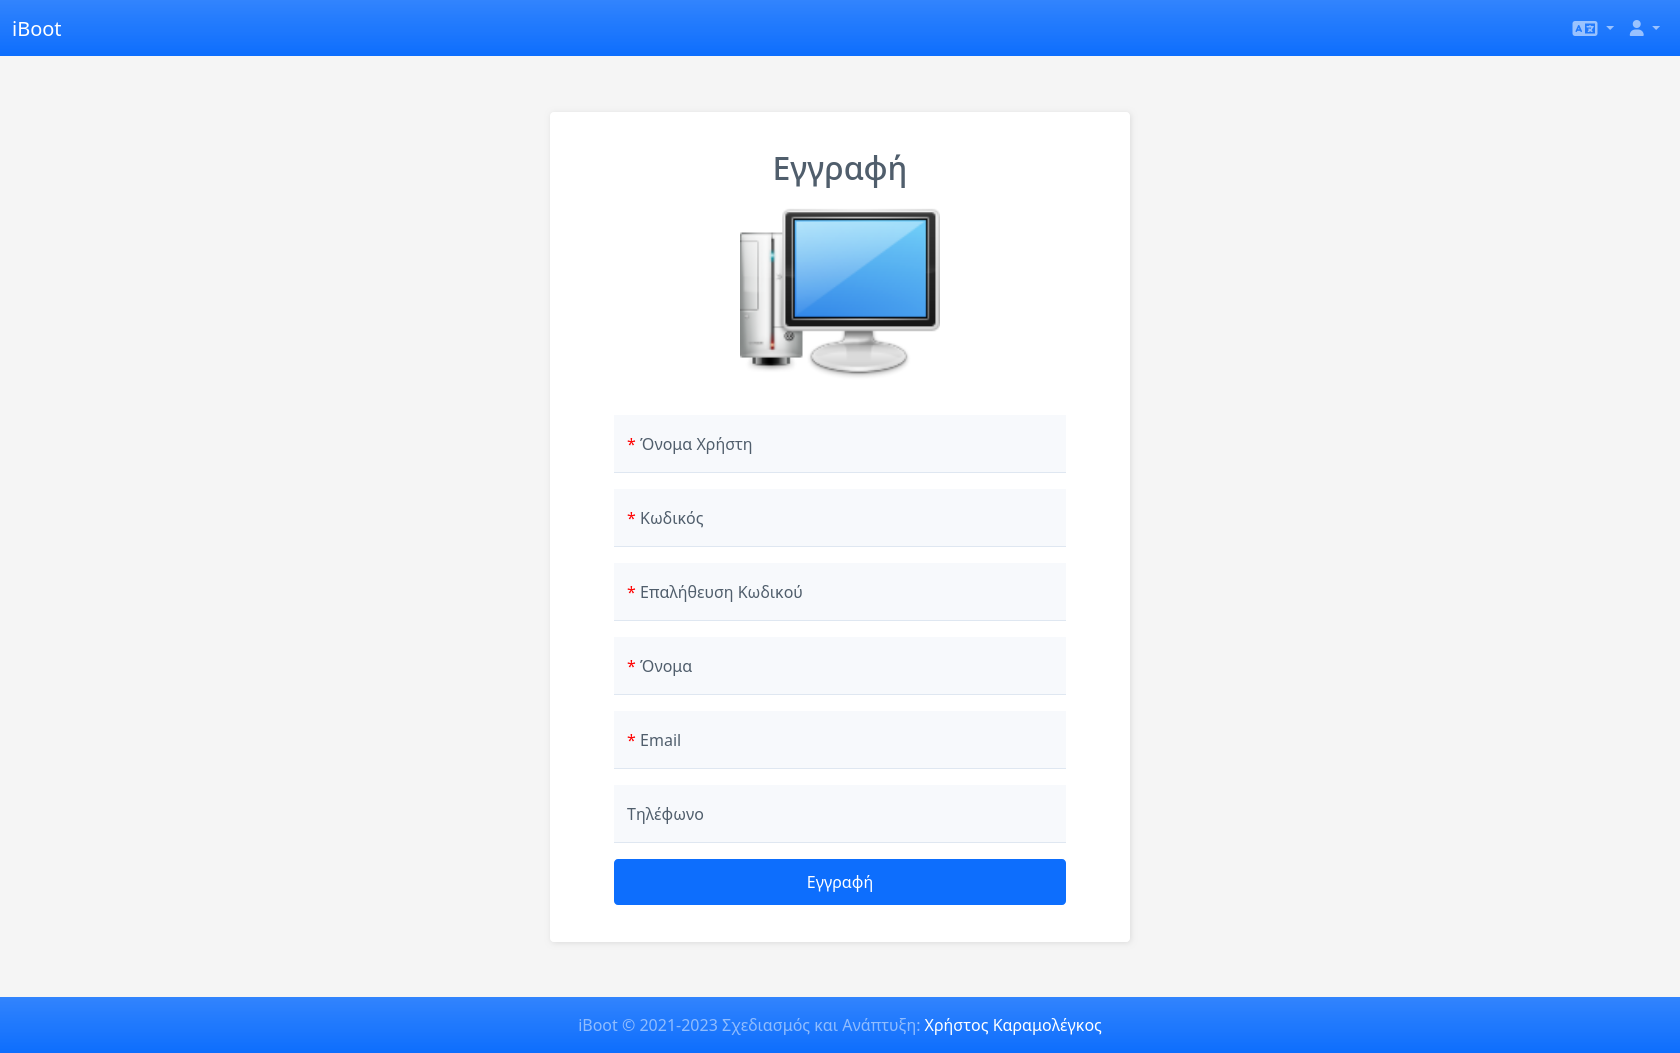
\includegraphics[scale=0.25]{iBoot-register.png}
	\caption{iBoot - Εγγραφή}
	\label{fig:iBoot_register}
\end{figure}

\begin{figure}[ht]
	\centering
	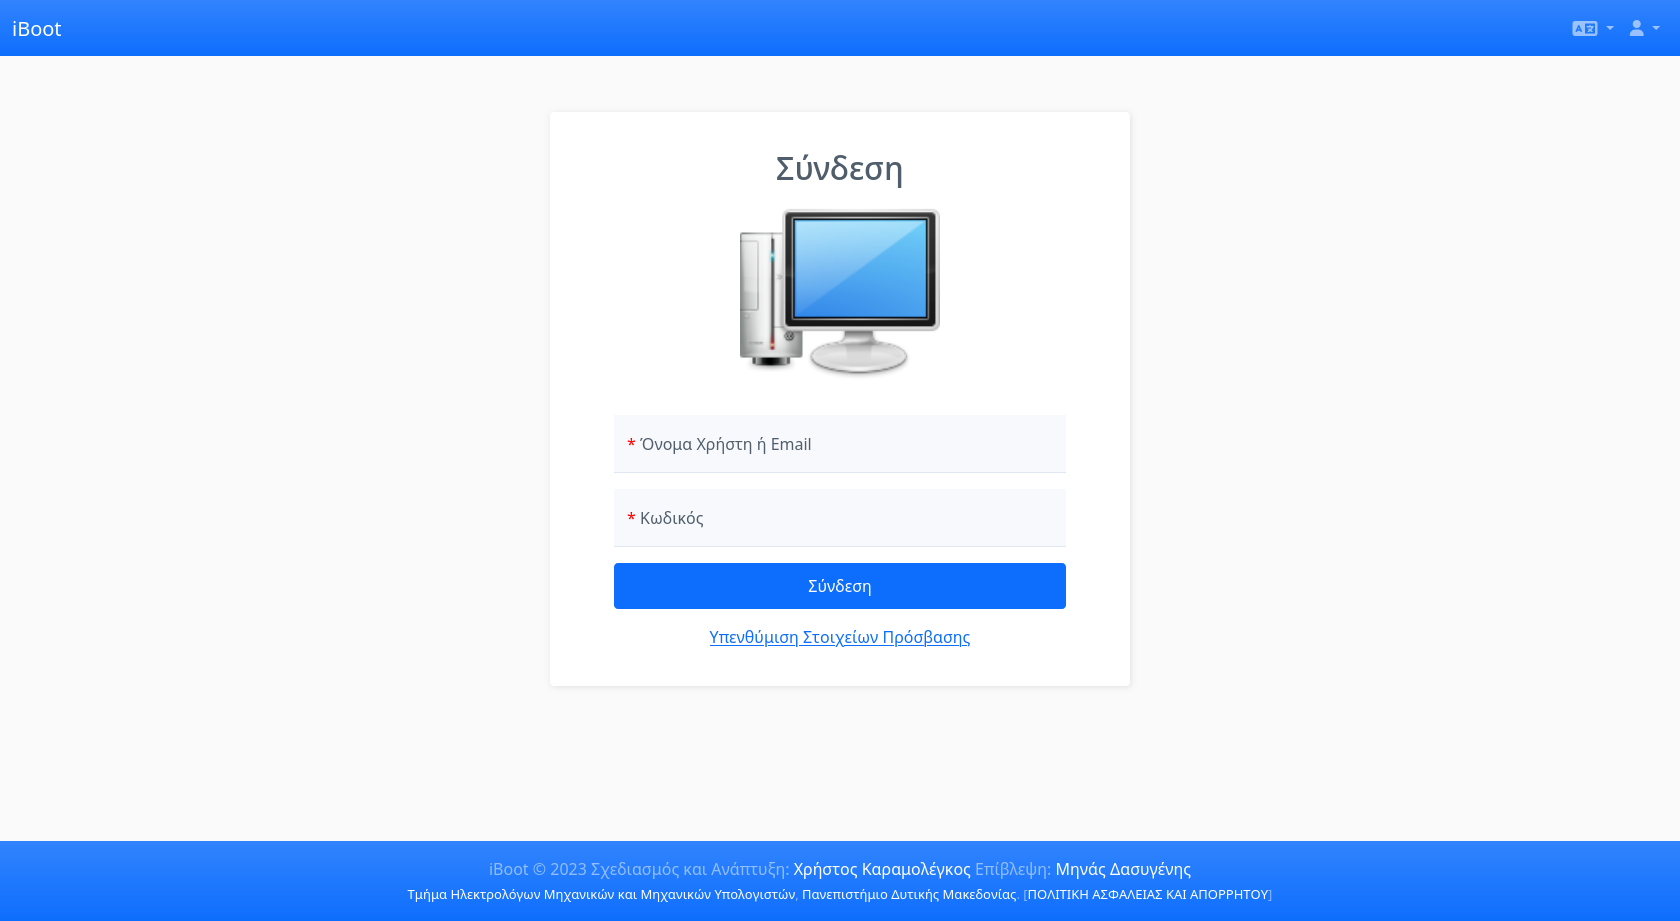
\includegraphics[scale=0.25]{iBoot-login.png}
	\caption{iBoot - Σύνδεση}
	\label{fig:iBoot_login}
\end{figure}

\begin{figure}[ht]
	\centering
	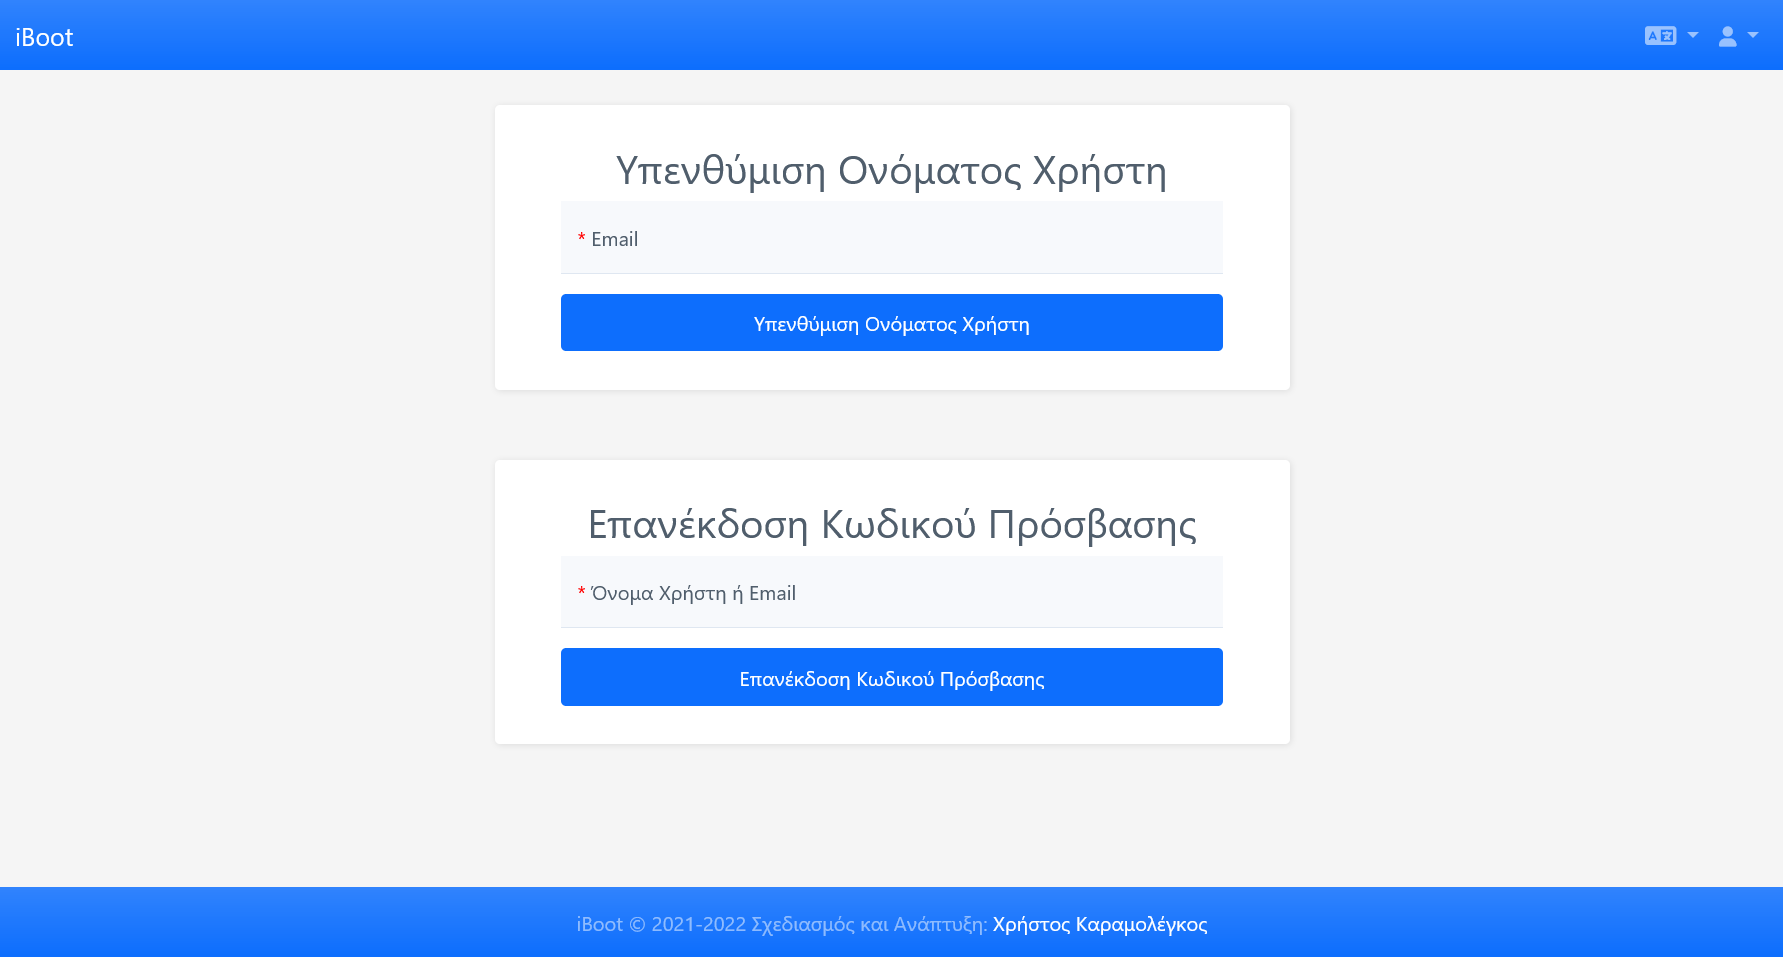
\includegraphics[scale=0.25]{iBoot-forgot-credentials.png}
	\caption{iBoot - Υπενθύμιση Στοιχείων Πρόσβασης}
	\label{fig:iBoot_forgot_credentials}
\end{figure}

\FloatBarrier

\subsection{Μενού Πλοήγησης}

\subsection{Υπολογιστές}

\subsection{Ομάδες Υπολογιστών}

\subsection{Εργαστήρια}

\subsection{Block εντολών τύπου ipxe}

\subsection{Μενού Εκκίνησης}

\subsection{Χρονοδιαγράμματα}

\subsection{Προδιαγραφή API}

\section{Επεξήγηση Αρχείων}
Καθώς η διαδικτυακή εφαρμογή αναπτύχθηκε με χρήση του CodeIgniter 4 Framework, χρησιμοποιεί και τη δομή αρχείων του.

\subsection{Βασική Δομή}
Η βασική δομή της εφαρμογής αποτελείται από πέντε καταλόγους: app/, public/, writable/, tests/ και vendor/ ή system/.

\subsection{app}
Στον κατάλογο app βρίσκεται όλος ο κώδικας της εφαρμογής. Οι ακόλουθοι φάκελοι αποτελούν τα βασικά περιεχόμενα:

\begin{forest}
	for tree={
		font=\ttfamily,
		grow'=0,
		child anchor=west,
		parent anchor=south,
		anchor=west,
		calign=first,
		inner xsep=7pt,
		edge path={
			\noexpand\path [draw, \forestoption{edge}]
			(!u.south west) +(7.5pt,0) |- (.child anchor) pic {folder} \forestoption{edge label};
		},
		before typesetting nodes={
			if n=1
			{insert before={[,phantom]}}
			{}
		},
		fit=band,
		before computing xy={l=15pt},
	}  
	[app/
		[Config/ \ \ \ \ \ \ \ \ Περιέχει τα αρχεία ρύθμισης παραμέτρων]
		[Controllers/ \ \ \ Περιέχει τους Controllers που καθορίζουν τη ροή του προγράμματος]
		[Database/ \ \ \ \ \ \ Περιέχει αρχεία για τη δημιουργία και ενημέρωση του σχήματος και την αρχικοποίηση βάσεων δεδομένων]
		[Filters/ \ \ \ \ \ \ \ Περιέχει κλάσεις φίλτρων που μπορούν να εκτελούνται πριν και μετά τους controllers]
		[Helpers/ \ \ \ \ \ \ \ Περιέχει συλλογές αυτόνομων βοηθητικών συναρτήσεων]
		[Language/ \ \ \ \ \ \ Περιέχει τις συμβολοσειρές γλώσσας για την υποστήριξη πολλαπλών γλωσσών]
		[Libraries/ \ \ \ \ \ Περιέχει χρήσιμες κλάσεις που δεν ταιριάζουν σε άλλη κατηγορία]
		[Models/ \ \ \ \ \ \ \ \ Περιέχει τα Models συνεργάζονται με τη βάση δεδομένων για την αναπαράσταση των επιχειρηματικών οντοτήτων]
		[ThirdParty/ \ \ \ \ Περιέχει βιβλιοθήκες τρίτων που μπορούν να χρησιμοποιηθούν στην εφαρμογή]
		[Views/ \ \ \ \ \ \ \ \ \ Περιέχει τα Views που συνθέτουν την HTML που εμφανίζεται στον πελάτη]
	]
\end{forest}

\subsection{public}

\subsection{writable}

\subsection{tests}

\subsection{system}

\section{Ασφάλεια Συστήματος}

\section{Σύνοψη Κεφαλαίου 4}
Στο κεφάλαιο 4, εξετάστηκαν όλες οι δυνατότητες της διαδικτυακής εφαρμογής και τα βήματα που πρέπει να ακολουθήσει ένας νέος χρήστης για να τις χρησιμοποιήσει. Επιπλέον, παρασχέθηκε οπτικό υλικό για κάθε λειτουργία στην οποία εμφανιζόταν στον χρήστη η διεπαφή χρήστη της διαδικτυακής εφαρμογής κατά την πλοήγησή του. Στη συνέχεια, εξηγήθηκαν διεξοδικά τόσο το front-end όσο και το back-end της δομής του πληροφοριακού συστήματος. Προκειμένου να διασφαλιστεί η ασφάλεια κατά τη χρήση της διαδικτυακής εφαρμογής, παρέχεται επεξήγηση των πρωτοκόλλων και των προσεγγίσεων ασφαλείας.

Στο επόμενο κεφάλαιο θα γίνει αξιολόγηση του συστήματος, ως προς την ορθή λειτουργία του και τις δυνατότητες κλιμάκωσής του.


\chapter{Αξιολόγηση Συστήματος}

\section{Δοκιμή Πλατφόρμας}

\section{Πλάνο Ελέγχου Ορθής Λειτουργίας}

\section{Μελέτη Κλιμάκωσης}


\chapter{Επίλογος}
Στο τελευταίο κεφάλαιο, πραγματοποιείται συνοπτική παρουσίαση των θεμάτων που αναλύθηκαν έως τώρα. Στη συνέχεια παρουσιάζονται τα συμπεράσματα που προέκυψαν κατά τη διαδικασία σχεδίασης και κατασκευής της διαδικτυακής εφαρμογής.
Επιπλέον, γίνεται λεπτομερής ανάλυση SWOT (Strengths, Weaknesses, Opportunities, Threats) του συστήματος, καθώς και προτάσεις για μελλοντικές βελτιστοποιήσεις και επεκτάσεις των λειτουργιών που παρέχει.

\section{Ανακεφαλαίωση Διπλωματικής Εργασίας}
Οι ανάγκες δικτυακής εκκίνησης υπολογιστών του Εργαστηρίου Ρομποτικής, Ενσωματωμένων και Ολοκληρωμένων Συστημάτων του Πανεπιστημίου Δυτικής Μακεδονίας, απαιτούσαν μια διαδικτυακή εφαρμογή με συγκεκριμένα χαρακτηριστικά και δυνατότητες που δεν ήταν διαθέσιμες σε εμπορικές λύσεις. Για την κάλυψη αυτών των αναγκών, αναπτύχθηκε η διαδικτυακή εφαρμογή `iBoot'.

Η εφαρμογή `iBoot' αναπτύχθηκε χρησιμοποιώντας PHP στο back-end και HTML, CSS, JavaScript και Bootstrap στο front-end. Τα δεδομένα της εφαρμογής αποθηκεύονται σε μια σχεσιακή βάση δεδομένων MySQL. Η πρόσβαση στην εφαρμογή μπορεί να γίνει είτε μέσω μιας διεπαφής χρήστη είτε μέσω ενός REST API που αναπτύχθηκε για αυτόν το σκοπό. Ο πηγαίος κώδικας της εφαρμογής είναι διαθέσιμος στο κοινό και έχει δημοσιευτεί υπό τους όρους της άδειας MIT.

Η εφαρμογή διευκολύνει την πρόσβαση σε τρεις τύπους χρηστών.

Ένας ανώνυμος χρήστης έχει πρόσβαση μόνο στις σελίδες σύνδεσης, εγγραφής και υπενθύμισης των διαπιστευτηρίων σύνδεσης.
Ο διαχειριστής εργαστηρίου μπορεί να διαχειρίζεται υπολογιστές σε συγκεκριμένα εργαστήρια. Μπορούν επίσης να τοποθετηθούν υπολογιστές σε εργαστήρια που διαχειρίζεται ο διαχειριστής και οι οποίοι δεν έχουν ήδη τοποθετηθεί σε άλλα εργαστήρια.
Ο διαχειριστής μπορεί να χρησιμοποιεί όλες τις δυνατότητες της πλατφόρμας χωρίς περιορισμούς. Ο διαχειριστής έχει την εξουσία να προσθέτει, να αφαιρεί και να τροποποιεί υπολογιστές, ομάδες, εργαστήρια, μπλοκ iPXE, μενού εκκίνησης, χρονοδιαγράμματα και χρήστες. Ο Διαχειριστής επιτρέπεται επίσης να βλέπει τα αρχεία καταγραφής συμβάντων της εφαρμογής.
Εν κατακλείδι,
Οι υπολογιστές επικοινωνούν με συγκεκριμένες σελίδες της εφαρμογής για να εγγραφούν και να λάβουν μενού εκκίνησης.

Η εφαρμογή έχει σχεδιαστεί και υλοποιηθεί σύμφωνα με τις βέλτιστες πρακτικές και τα πιο πρόσφατα πρότυπα ασφαλείας για την προστασία των πληροφοριών που περιέχονται σε αυτήν. Οι κωδικοί πρόσβασης των χρηστών αποθηκεύονται στη βάση δεδομένων της εφαρμογής αφού υποστούν επεξεργασία μέσω κρυπτογραφικά ασφαλών συναρτήσεων κατακερματισμού και δεν εμφανίζονται ποτέ στην εφαρμογή. Η πιστοποίηση ταυτότητας και τα δικαιώματα του χρήστη που επιθυμεί να προβάλει τη σελίδα ελέγχονται πριν από τη φόρτωση, ενώ το API υλοποιεί την ίδια διαδικασία προσθέτοντας σε κάθε αίτηση JWT tokens. Η εφαρμογή είναι σε θέση να λειτουργεί τόσο με το πρωτόκολλο HTTP όσο και με το πιο ασφαλές πρωτόκολλο HTTPS και μπορεί ακόμη και να κρυπτογραφήσει τα cookies συνόδου.

Το Εργαστήριο Ρομποτικής, Ενσωματωμένων και Ολοκληρωμένων Συστημάτων του Πανεπιστημίου Δυτικής Μακεδονίας θα εκσυγχρονίσει τη διαδικασία διαχείρισης του μενού εκκίνησης του δικτύου των υπολογιστών του με την εγκατάσταση της διαδικτυακής εφαρμογής "iBoot", η οποία θα διευκολύνει επίσης σημαντικά την καταγραφή και την παρακολούθηση των υπολογιστών αυτών.

\section{Μοντέλο Ανάλυσης S.W.O.T.}

\subsection{Ορισμός Μοντέλου Ανάλυσης S.W.O.T.}
Η ανάλυση SWOT, ή πίνακας SWOT, είναι ένα εργαλείο στρατηγικού σχεδιασμού και διαχείρισης που χρησιμοποιείται για να επιτρέψει σε άτομα ή οργανισμούς να εντοπίσουν τα δυνατά σημεία, τις αδυναμίες, τις ευκαιρίες και τις απειλές που σχετίζονται με τον επιχειρηματικό ανταγωνισμό ή τον προγραμματισμό έργων.

Η τεχνική αυτή προορίζεται για χρήση κατά τα προκαταρκτικά στάδια των διαδικασιών λήψης αποφάσεων για την αξιολόγηση της στρατηγικής θέσης. Σκοπός της είναι να εντοπίσει τόσο εσωτερικούς όσο και εξωτερικούς παράγοντες που είναι είτε ευνοϊκοί είτε δυσμενείς για την επίτευξη των στόχων του έργου ή της πρωτοβουλίας.

Ο όρος αποτελεί ακρωνύμιο των τεσσάρων στοιχείων τα οποία αξιολογεί η μέθοδος:

\begin{description}
	\item[Δυνάμεις:] χαρακτηριστικά της επιχείρησης ή του έργου που παρέχουν πλεονέκτημα έναντι του ανταγωνισμού
	\item[Αδυναμίες:] χαρακτηριστικά που θέτουν την επιχείρηση ή το έργο σε μειονεκτική θέση σε σχέση με τον ανταγωνισμό
	\item[Ευκαιρίες:] παράγοντες του περιβάλλοντος που μπορεί να εκμεταλλευτεί η επιχείρηση ή το έργο
	\item[Απειλές:] παράγοντες του περιβάλλοντος που θα μπορούσαν να αποτελέσουν προκλήσεις για την επιχείρηση ή το έργο
\end{description}

Τα αποτελέσματα της αξιολόγησης εμφανίζονται συνήθως είτε σε μορφή πίνακα είτε σε παραγράφους.

\subsubsection{Εσωτερικοί - Εξωτερικοί Παράγοντες}
Οι εσωτερικές πτυχές μιας επιχείρησης θεωρούνται συνήθως ως πλεονεκτήματα ή αδυναμίες, ενώ οι ευκαιρίες ή οι απειλές θεωρούνται ως εξωτερικές.

Οι εσωτερικοί παράγοντες ενός οργανισμού αξιολογούνται ως πλεονεκτήματα ή αδυναμίες, με βάση τον αντίκτυπό τους στους στόχους της επιχείρησης. Κάτι που θα μπορούσε να θεωρηθεί ως πλεονέκτημα για έναν στόχο μπορεί να θεωρηθεί ως αδυναμία για έναν άλλο, για παράδειγμα, ο ανταγωνισμός ή οι περισπασμοί. Οι παράγοντες μπορεί να περιλαμβάνουν το προσωπικό, τη χρηματοδότηση, τις δυνατότητες παραγωγής και όλα τα 4P του μείγματος μάρκετινγκ (προϊόν, τιμή, θέση και προώθηση).

Οι εξωτερικοί παράγοντες περιέχουν κοινωνικοπολιτισμικές αλλαγές, μακροοικονομικές εξελίξεις, νομοθετικές εξελίξεις, τεχνολογικές εξελίξεις, καθώς και μετατοπίσεις στην αγορά.

\subsection{Ανάλυση S.W.O.T. εφαρμογής iBoot}
Στο σχήμα \ref{fig:iBoot_swot_analysis} απεικονίζεται η ανάλυση S.W.O.T. της διαδικτυακής εφαρμογής iBoot. Τα ευρήματα της ανάλυσης αναλύονται στη συνέχεια, το καθένα στην αντίστοιχη υποενότητα.

\begin{figure}[ht]
	\centering
	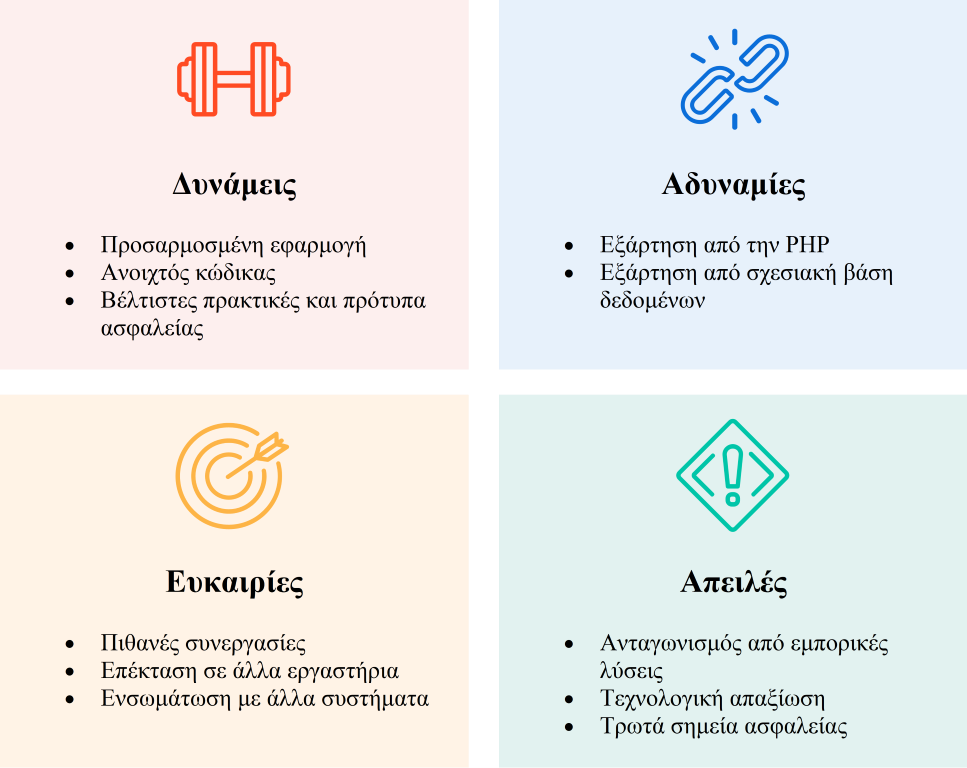
\includegraphics[scale=0.5]{swot-analysis.png}
	\caption{Ανάλυση SWOT εφαρμογής iBoot}
	\label{fig:iBoot_swot_analysis}
\end{figure}

\subsubsection{Δυνάμεις}
\begin{description}
	\item[Προσαρμοσμένη εφαρμογή:] Η εφαρμογή iBoot αναπτύχθηκε ειδικά για να ανταποκρίνεται στις απαιτήσεις του Εργαστηρίου Ρομποτικής, Ενσωματωμένων και Ολοκληρωμένων Συστημάτων, διασφαλίζοντας ότι διαθέτει τα απαραίτητα χαρακτηριστικά και δυνατότητες.
	\item[Ανοιχτός κώδικας:] Ο πηγαίος κώδικας της εφαρμογής είναι διαθέσιμος στο κοινό και δημοσιεύεται με την άδεια MIT, επιτρέποντας τη διαφάνεια και τις πιθανές συνεισφορές της κοινότητας.
	\item[Βέλτιστες πρακτικές και πρότυπα ασφαλείας:] Η εφαρμογή έχει σχεδιαστεί και υλοποιηθεί σύμφωνα με τις βέλτιστες πρακτικές και τα πιο πρόσφατα πρότυπα ασφαλείας, διασφαλίζοντας την προστασία των πληροφοριών και την κρυπτογράφηση των cookies συνόδου.
\end{description}

\subsubsection{Αδυναμίες}
\begin{description}
	\item[Εξάρτηση από την PHP:] Το back-end της εφαρμογής iBoot είναι κατασκευασμένο με τη χρήση PHP, η οποία μπορεί να δημιουργήσει προκλήσεις όσον αφορά την επεκτασιμότητα και τη συμβατότητα με μελλοντικές τεχνολογίες.
	\item[Εξάρτηση από σχεσιακή βάση δεδομένων:] Η εφαρμογή βασίζεται σε μια σχεσιακή βάση δεδομένων MySQL για την αποθήκευση δεδομένων, γεγονός που ενδέχεται να περιορίσει την επεκτασιμότητα και την απόδοση κατά τον χειρισμό μεγάλων όγκων δεδομένων.
\end{description}

\subsubsection{Ευκαιρίες}
\begin{description}
	\item[Πιθανές συνεργασίες:] Η φύση της εφαρμογής ως ανοικτού κώδικα δημιουργεί ευκαιρίες συνεργασίας με άλλα ιδρύματα ή προγραμματιστές που μπορούν να συμβάλουν στην περαιτέρω βελτίωσή της.
	\item[Επέκταση σε άλλα εργαστήρια:] Η επιτυχία και ο θετικός αντίκτυπος της εφαρμογής iBoot στο Εργαστήριο Ρομποτικής, Ενσωματωμένων και Ολοκληρωμένων Συστημάτων μπορεί να οδηγήσει στην υιοθέτησή της από άλλα εργαστήρια εντός του Πανεπιστημίου Δυτικής Μακεδονίας ή και πέραν αυτού.
	\item[Ενσωμάτωση με άλλα συστήματα:] Η εφαρμογή μπορεί να διερευνήσει ευκαιρίες για ενσωμάτωση με άλλα συστήματα ή πλατφόρμες, επιτρέποντας βελτιωμένη λειτουργικότητα και διαλειτουργικότητα.
\end{description}

\subsubsection{Απειλές}
\begin{description}
	\item[Ανταγωνισμός από εμπορικές λύσεις:] Παρόλο που η εφαρμογή iBoot αναπτύχθηκε για να ικανοποιήσει συγκεκριμένες απαιτήσεις, υπάρχει πιθανότητα ανταγωνισμού από εμπορικές λύσεις που μπορεί να προσφέρουν περισσότερα χαρακτηριστικά ή ευρύτερο φάσμα δυνατοτήτων.
	\item[Τεχνολογική απαξίωση:] Οι ταχείες εξελίξεις στην τεχνολογία ενδέχεται να καταστήσουν ορισμένες πτυχές της εφαρμογής ξεπερασμένες, απαιτώντας συνεχείς ενημερώσεις και προσαρμογές για να παραμείνει επίκαιρη.
	\item[Τρωτά σημεία ασφαλείας:] Παρά την τήρηση των βέλτιστων πρακτικών και των προτύπων ασφαλείας της εφαρμογής, υπάρχει ο κίνδυνος τρωτών σημείων ασφαλείας και πιθανών παραβιάσεων, οι οποίες θα μπορούσαν να θέσουν σε κίνδυνο τις πληροφορίες και τη λειτουργικότητα της εφαρμογής.
\end{description}

\section{Μελλοντικές Επεκτάσεις}
Όλες οι διαδικτυακές εφαρμογές οφείλουν να αναβαθμίζονται συνεχώς ώστε, πέρα από την προσθήκη νέων δυνατοτήτων και τη βελτίωση των υπαρχόντων, να παραμένουν λειτουργικές και ασφαλείς. Συχνά χρειάζεται επίσης και η ενημέρωση βιβλιοθηκών και άλλων εξαρτήσεων της εφαρμογής, ώστε να καλύπτονται πιθανά κενά ασφαλείας και να επιλύονται προβλήματα που ίσως υπάρχουν. Η διαδικτυακή εφαρμογή που αναπτύχθηκε δεν αποτελεί εξαίρεση. Η βιωσιμότητα της είναι άμεσα εξαρτώμενη από τις εργασίες συντήρησης και ενημέρωσης της, οι οποίες θα πρέπει να πραγματοποιούνται τακτικά.

Μερικές ιδέες για περαιτέρω ανάπτυξη της εφαρμογής παρουσιάζονται στη συνέχεια.

\begin{description}
	\item[Διεύρυνση λειτουργιών του REST API:] To REST API θα μπορούσε να διευρυνθεί, προσθέτοντας endpoints που θα προσφέρουν διαλειτουργικότητα με άλλες εφαρμογές και υπηρεσίες. Αν αξιολογηθεί ως σημαντικό, θα μπορούσαν να προστεθούν συναρτήσεις ανάκτησης τμήματος δεδομένων, με περισσότερους ελέγχους πρόσβασης. Τέλος, θα ήταν ίσως χρήσιμη η προσθήκη μιας προαιρετικής παραμέτρου σελιδοποίησης, ώστε να αντλείται συγκεκριμένος αριθμός εγγραφών από την κάθε κλήση στα endpoints του API. Κάτι τέτοιο θα βελτίωνε την απόδοση της εφαρμογής σε μεγάλους αριθμούς εγγραφών.
	\item[Ανάπτυξη εναλλακτικών front-end:] Η ύπαρξη του REST API ευνοεί τη δημιουργία εναλλακτικών front-end για την εφαρμογή, αφού ουσιαστικά το front-end με το back-end είναι αποσυνδεδεμένα και επικοινωνούν μέσω του API της εφαρμογής. Ένα εναλλακτικό front-end θα μπορούσε να προσφέρει μεγαλύτερη συμβατότητα με συγκεκριμένους τύπους συσκευών, να εμφανίζει τις πληροφορίες της εφαρμογής με έναν πιο μοντέρνο και παραμετροποιήσιμο τρόπο, ή ακόμη και να πακεταριστεί σε εγγενή εφαρμογή για κάποιο λειτουργικό σύστημα υπολογιστών.
	\item[Υποστήριξη διαφορετικών μεθόδων αυθεντικοποίησης:] Η εγγραφή και σύνδεση στο σύστημα θα μπορούσε να αξιοποιεί υπάρχοντα πρωτόκολλα διαπιστευτηρίων, ώστε να υποστηρίζεται και η διαλειτουργικότητα με την υπόλοιπη υποδομή κάποιου εργαστηρίου. Τέτοια πρωτόκολλα είναι τα LDAP, OAuth2, SAML και άλλα. Επίσης, θα μπορούσε να αναπτυχθεί υποστήριξη για σύνδεση με χρήση πολλαπλών παραγόντων ή και σύνδεσης χωρίς κωδικό πρόσβασης με magic link στο email του χρήστη.
	\item[Προσθήκη λειτουργίας Wake-On-Lan:] Θα μπορούσε να διερευνηθεί η δυνατότητα δημιουργίας και αποστολής Wake-On-Lan πακέτων στο δίκτυο των υπολογιστών, ώστε η διαδικασία εκκίνησής τους να μπορεί να ξεκινήσει απευθείας από την εφαρμογή και χωρίς φυσική πρόσβαση στο κάθε μηχάνημα.
	\item[Τροποποίηση ημερολογίου σε επεξεργάσιμο:] Το ημερολόγιο των χρονοδιαγραμμάτων θα μπορούσε να γίνει επεξεργάσιμο και έτσι δημιουργία νέων  ή η τροποποίηση υπαρχόντων χρονοδιαγραμμάτων να γίνεται απευθείας σε αυτό.
	\item[Προσθήκη δυνατότητας ανακατάταξης των Μπλοκ iPXE:] Θα μπορούσε να προστεθεί η δυνατότητα ανακατάταξης των Μπλοκ iPXE μέσα σε κάθε μενού, ώστε ο χρήστης να μπορεί να αλλάξει τη σειρά με την οποία εμφανίζονται κατά την εκκίνηση υπολογιστών, αντί για την μη-παραμετροποιήσιμη σειρά απεικόνισης που υπάρχει τώρα, καταταγμένη βάση της χρονολογικής σειράς με την οποία προστέθηκαν τα Μπλοκς στο κάθε μενού.
	\item[Ενσωμάτωση relay DHCP server:] Η εφαρμογή θα μπορούσε να ενσωματώσει έναν relay DHCP server, ώστε να μπορεί να εγκατασταθεί στο τοπικό δίκτυο και να λειτουργήσει χωρίς επεξεργασία των ρυθμίσεων του προϋπάρχοντος DHCP server του δικτύου.
\end{description}

\section{Συμπεράσματα}


\section{Σύνοψη Κεφαλαίου 6}
Το κεφάλαιο 6 σηματοδοτεί το πέρας της παρούσας διπλωματικής εργασίας. Στο παρόν κεφάλαιο παρέχεται μια ανάλυση SWOT του περιεχομένου της διαδικτυακής πλατφόρμας, η οποία περιγράφει συνοπτικά τα πλεονεκτήματα και τα μειονεκτήματα που σχετίζονται με την υλοποίηση του παρόντος έργου, καθώς και τις δυνατότητες και τα οφέλη που παρουσιάζει και τυχόν πιθανούς κινδύνους που μπορεί να αντιμετωπίσει. Παρέχονται επίσης ορισμένες ιδέες για πιθανές μελλοντικές βελτιώσεις και προσαρμογές της πλατφόρμας. Το κεφάλαιο αυτό ολοκληρώνεται με τα τελικά συμπεράσματα επί της διπλωματικής εργασίας.


\begin{appendices}

\end{appendices}

{\footnotesize
	\printbibliography[title={Βιβλιογραφία}]
}

\end{document} 
